\chapter{Umsetzung}
\label{cha:Umsetzung}

Die Reihenfolge der hier aufgezählten Punkte richtet sich grob nach der
chronologischen
Reihenfolge, in der diese abgearbeitet wurden.
Teilweise greifen unterschiedliche Aspekte ineinander, sodass in diesem Fall der
Punkt, der die Grundlage für einen anderen Punkt ist, als Erstes erwähnt wird.

\section{Analyse der Ausgangssituation}

\subsection{Hardware}

Bei der Anwendung, die migriert werden soll, handelt es sich um mehrere
Komponenten.
Diese sind vor der Migrierung mittels Ansible auf einem \$ 80,- / Monat
Digital Ocean Server \cite{digitalocean} installiert worden.
Dieser Server ist relativ leistungsfähig, damit die Lastspitzen abgefangen
werden können.
Die konkrete Spezifikation dieses Servers ist: Quad Core, 8 GB Ram und 80 GB SSD
Festplatte.

\subsection{Software}
Mit einer Reihe von Ansible Playbooks wurden folgende Komponenten deployed.

\subsubsection{API}
Die API ist eine \emph{NodeJS} Applikation \cite{nodejs} mit REST Schnittstelle.
Um Daten zu persistieren, verwendet
die Applikation eine dahinter liegende PostgreSQL-Datenbank.
Es laufen 4 Prozesse auf den 4 Prozessor-Kernen.

\subsubsection{Loadbalancer}
Ein Nginx-Prozess verteilt die Last gleichmäßig auf die zur Verfügung
stehenden API-Endpoints.
Zudem kann hier die TLS-Termination für HTTPS stattfinden.

\subsubsection{Datenbank}
PostgreSQL Datenbank \cite{postgresql}, in der Daten über die API abgespeichert und abgerufen werden.

\subsubsection{Website}
Über Apache werden hier größtenteils statische Inhalte (HTML, JavaScript und
CSS) ausgeliefert.
Dynamische Inhalte werden mittels JavaScript über die API nachgeladen.

\subsection{Benutzungs-Profil}
Das Charakteristische am Benutzungs-Profil dieser Anwendung,
ist, dass sie während des Monats nur relativ geringe Benutzerzahlen verzeichnet.
Am letzten
Freitag jedes Monats steigt die Benutzerzahl dann aber dramatisch an.
Die Anwendung dient dazu, einen Fahrrad-Protest zu organisieren,
der weltweit in unterschiedlichen Städten stattfindet, wobei der Zeitpunkt immer
der letzte Freitag des Monats ist.

An diesen Tagen nutzen circa 2.500 Menschen die Android App, circa 2.000 Menschen benutzen die iPhone App
und circa 1.000 Menschen die Website.
Da jede Client-Applikation immer Echtzeit-Daten darstellen soll, fragen die Clients
alle 20 Sekunden, also 3 pro Minute, neue Daten von der API an.
Zu diesem Peak-Zeiten muss also mit circa
\\\code{(2.500 + 2.000 + 1.000) * 3 = 16.500} \\Requests pro Minute (RPM) gerechnet werden.

\section{Technologie Stack}

Die hier aufgeführten Elemente sind nach eingehender Recherche ausgewählt und im
Vorfeld dieser Arbeit schon einzeln ausprobiert worden.
Ziel dieser Arbeit soll es nun sein, diese einzelnen Komponenten im Zusammenspiel
praktisch zu erproben und deren Tauglichkeit für den Betrieb in einem
Kubernetes-Cluster festzustellen.

\subsection{Kubernetes}

Kubernetes steht im Zentrum dieser Arbeit und legt somit auch die Grundlage
für die weitere Auswahl der Technologien. Aus diesem Grund soll an dieser Stelle
besonders detailliert auf Kubernetes eingegangen werden.

Das interne Google Tool \quotes{Borg}, wurde im Juni 2016 auf Github der
Open Source Community unter dem Namen \quotes{Kubernetes}
(kurz: \quotes{k8s}; altgriechisch für \quotes{Steuermann}) zur Verfügung gestellt.
Google sammelt schon seit über einer Dekade Erfahrungen im Bereich des Managements
großer Container Cluster in Produktions-Systemen mit dieser Software \cite{borg}.
Dieser
Erfahrungsschatz ist nun mit Kubernetes der Open Source Community zugänglich
und wird mit großem
Enthusiasmus entgegen genommen.
So hat Kubernetes zum Stichtag 27. Januar 2017 folgende Kennzahlen \cite{k8srepo} vorzuweisen:
\begin{itemize}
  \item 42.710 Commits
  \item 1.057 Contributors
  \item 594 offene Pull requests
  \item 4.977 offene Issues
\end{itemize}
Es ist damit eines der populärsten Repositories auf Github.
Hieran ist auch zu erkennen, dass zahlreiche
Menschen die Möglichkeit in Anspruch nehmen, selbst einen Beitrag zu diesem
Projekt zu leisten.
Auch das herausragende Community-Management von Google zu diesem Projekt
hat sicher zu diesem
großen Zulauf beigetragen.

Kubernetes füllt damit auch eine Lücke in der Auswahl an Container Orchestration
Tools, die vorher nicht besetzt wurde von Tools wie Docker Swarm oder Apache Mesos.
Ohne genauer auf die Unterschiede einzugehen, lässt sich sagen, dass Kubernetes
in Sachen Komplexität und Features zwischen dem komplexen und sehr flexiblen
\emph{Apache Mesos} und dem eher einfachen und starren \emph{Docker Swarm} zu verorten ist.

Mit folgendem Vergleich der Suchanfragen für die jeweiligen Orchestration-Tools,
soll verdeutlicht werden, wie stark das Interesse an Kubernetes auch im Vergleich
zu seinen Haupt-Konkurrenten angestiegen ist.

\begin{figure}[H]
\centering
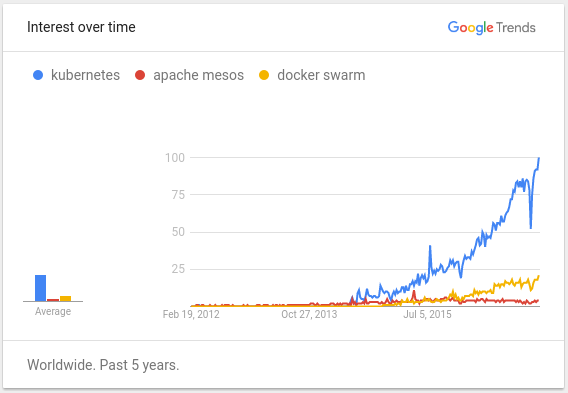
\includegraphics[width=0.8\textwidth]{trends}
\caption{Vergleich der Suchanfragen zu Orchestrierungs-Tools mit Google Trends \cite{trends}}
\end{figure}

\subsubsection{Was ist Kubernetes?}

Kubernetes ist Software, die auf mehreren Servern installiert wird und dazu dient,
Prozesse, die in Containern laufen, zu verwalten. Anstatt diese Container und
Server alle einzeln zu verwalten, bietet Kubernetes abstrahierte Schnittstellen an,
über die das gesamte Cluster bedient werden kann, als wäre es eine Einheit.

Kubernetes löst einige der Probleme des Betriebes eines Clusters selbst und
bietet für
andere diverse Schnittstellen für Plugins und Addons.

Im Folgenden soll auf die elementaren Konzepte und grundlegenden Features
eines Kubernetes-Cluster
eingegangen werden, damit diese für
die Umsetzung geklärt sind.

\subsubsection{Konzepte}

\begin{description}
  \item[Nodes:]
  Ein Node kann ein \emph{Bare Metal Server} oder eine virtuelle Maschine
  in der Cloud oder auf dem lokalen Computer sein.
  Kubernetes unterscheidet zwischen zwei unterschiedlichen Arten von Nodes. Die
  \textbf{Master Node} ist die Node, auf der die Software installiert ist,
  die das Cluster kontrolliert und steuert. Auf den \textbf{Worker Nodes} laufen
  Workloads, die die
  eigentliche Domain-Logik bereit stellen. Über \emph{Node Labels} können
  Worker Nodes getaggt werden, sodass ihnen später spezielle Aufgaben
  zugewiesen werden können.
  \item[Manifeste:]
  Manifeste sind die Konfigurations-Dateien im YAML- oder JSON-Format, mit denen
  die einzelnen Komponenten des Clusters an die Kubernetes-API
  übermittelt werden.
  \item[Pods:]
  Pods sind eine oder mehrere Container, die derselbe Lifecycle verbindet.
  Sie werden gemeinsam platziert und finden ihre offenen Ports auf dem selben
  \code{localhost} Interface.
  Sie können über Volumes auch gemeinsame Ordner und Dateien bearbeiten.
  Ein simples Manifest eines Pods sieht dann beispielsweise so aus:
  \begin{lstlisting}[language=Python,numbers=none]
  apiVersion: v1
  kind: Pod
  metadata:
    name: api
    labels:
      app: api
  spec:
    containers:
    - name: api
      image: nodejs-image
      ports:
      - containerPort: 8080
    - name: mysql
      image: mysql-image
      ports:
      - containerPort: 3306  \end{lstlisting}

  \item[Service:]
  Services werden benutzt, um Pod-Ressourcen nach außen hin oder cluster-intern
  zu exponieren.
  Sie übernehmen außerdem die Funktion eines Load-Balancers.
  Services sind deshalb eine weitere Abstraktion des Pod-Interfaces, da Pods als
  kurzlebige Prozesse betrachtet werden. Ein Pod kann jederzeit terminiert werden
  und mit einer neuen Cluster-IP an einer anderen Stelle wieder gestartet werden.
  Ein Service sorgt mittels \emph{iptables} und den Proxies auf den Nodes dafür,
  dass er immer als Load Balancer auf alle verfügbaren Pods fungiert.
  Als Standardeinstellung verteilt ein Service die Requests per \emph{Round Robin}
  auf die verfügbaren Backend-Pods. \cite{networkingBla}

  Eine Konfiguration, die den Beispiel-Pod selektiert, sieht dann
  folgendermaßen aus:
  \begin{lstlisting}[language=Python,numbers=none]
  apiVersion: v1
  kind: Service
  metadata:
    name: api-service
    labels:
      name: api-service
  spec:
    ports:
    - port: 80
      targetPort: 8080
    selector:
      app: api \end{lstlisting}

  Dieser Zusammenhang stellt sich dann mit mehreren Pods grafisch
  folgendermaßen dar:
  \begin{figure}[H]
  \centering
  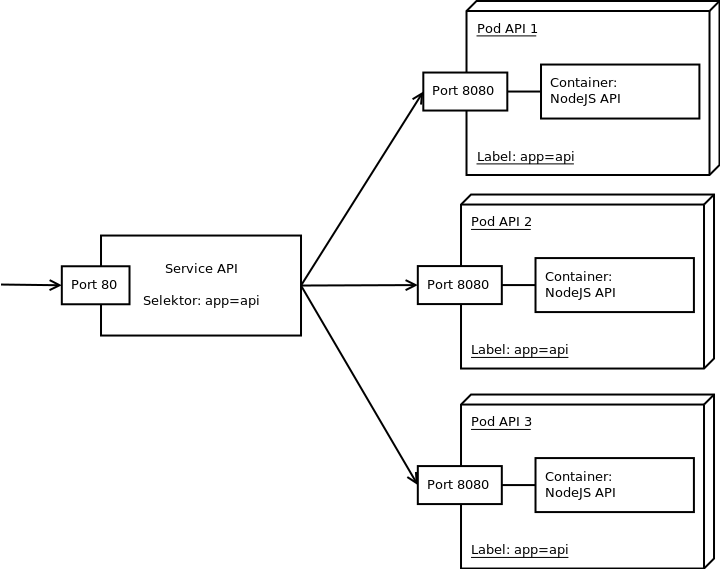
\includegraphics[width=0.8\textwidth]{service}
  \caption{Beispielhaftes Zusammenspiel zwischen einem Service und mehreren Pods}
  \end{figure}
  \item[Replication Controller:]
  Ein \emph{Replication Controller} wacht darüber, dass im Cluster immer eine
  bestimmte Anzahl an Pods laufen. Sollte ein Pod terminieren, startet der
  \emph{Replication Controller} einen neuen.
  \item[Deployments:]
  Wie ein \emph{Replication Controller}, nur mit der  zusätzlichen
  Funktionalität, neue Image-Versionen per
  \emph{Rolling Update} zu starten, anstatt alle zum gleichen Zeitpunkt zu stoppen
  und erst dann wieder
  mit neuem Image zu starten. So kann eine Downtime dieses Services umgangen
  werden.

\end{description}

\subsubsection{Features}

\begin{description}
  \item[Portabilität:]
  Kubernetes kann auf einer Vielzahl von Linux-Distributionen
  (wie Ubuntu, Fedora, Debian, CentOS oder CoreOS) installiert werden.
  Es ist damit
  größtenteils unabhängig von dem darunter liegenden IaaS-Provider. Ein Umzug
  auf ein
  anderes darunter liegendes Betriebssystem würde dann bedeuten,
  dass Kubernetes
  auf den neuen Servern installiert werden muss. Danach müssen nur noch
  die alten Konfigurations-Dateien auf das neue Cluster angewendet werden.
  \item[Service Discovery:]
  Bei dem Discovery Service geht es darum, Ressourcen, die sich nicht immer an einer
  statischen
  Adresse befinden, zu finden. So müssen sich zum Beispiel Services, deren IP
  dynamisch vergeben wird,
  von der konsumierenden Instanz (beispielsweise einem Load Balancer) auch
  gefunden werden.
  In Kubernetes bekommen diese dynamischen Instanzen ein Label, mit dem der
  konsumierende Service sie
  mittels eines Selektors auf dieses Label erkennt.
  \item[Self Healing:]
  Sollte ein Container aufgrund diverser Metriken als fehlerhaft
  identifiziert werden,
  kümmert sich
  Kubernetes darum, dass dieser Pod terminiert wird und ein neuer
  funktionierender Pod gestartet wird.
  Wenn eine komplette Node ausfallen sollte, werden die sich darauf befindenden
  Pods, auf einer anderen Node gestartet.
  \item[Bin Packing:]
  Pods können mit bestimmten Anforderungen an Ressourcen definiert werden.
  Kubernetes weiß um
  die zur Verfügung stehenden Ressourcen auf den einzelnen Nodes und kann
  dementsprechend
  Entscheidungen treffen, wo diese Pods platziert werden sollen. So werden die
  vorhandenen
  Ressourcen effizient genutzt.
  \item[Load Balancing:]
  Die Endpoints der Pods werden über Services an konsumierende Services nach
  außen oder cluster-intern freigegeben. Der Service bietet die Pods an, die dem
  Selektor entsprechen, mit der er konfiguriert wurde. Sollte es mehr als einen
  Pod geben,
  dessen Label dem Selektor des Services entspricht, wird der eingehende
  Traffic auf diese Pods verteilt.
  Eine weitere Möglichkeit Loadbalancing zu betreiben, ist, über eine
  Ingress-Ressource,
  welche ein Wrapper um Nginx ist. Dieser verteilt die Last auf verschiedene Pods
  und
  konfiguriert sich neu, sollte es Änderungen bezüglich der Backend-Pods geben.
  Ingress-Ressourcen können zudem auch weitere Features von Nginx übernehmen,
  wie die TLS-Termination, Basic-Auth oder die Verteilung der Requests auf Grundlage
  der angefragten Domains und Pfade.
  \item[Auto-Scaling:]
  Der \emph{Horizontal Pod Autoscaler} kann, auf Grundlage der konsumierten CPU-Leistung
  oder des verwendeten Arbeitsspeichers eines
  Replication Controllers oder Deployments, neue Pods starten, sodass die benötigten
  Ressourcen pro Pod im Durchschnitt wieder sinken. Sollte die
  Ressourcen-Nachfrage dann wieder sinken,
  wird auch dem Rechnung getragen, indem Pods wieder gestoppt werden. Um nicht ins
  Unendliche zu skalieren und, um nicht unter eine Pod-Anzahl zu gelangen, die
  die Ausfallsicherheit gefährdet, können Minimums und Maximums festgelegt werden.
  \item[Persistenz:] Da Pods kurzlebige Prozesse sind, die keine Daten selbst
  speichern, gibt es in Kubernetes die Möglichkeiten, diese Daten
  persistent abzulegen.
  Pods können dann ihre Daten in \emph{Persistent Volumes} ablegen, wo sie auch, wenn
  der Pod terminiert,
  weiterhin zur Verfügung stehen. Ein Datenbank-Container, kann also terminieren
  und findet, nachdem er wieder gestartet wurde dieselben alten Daten
  in diesem Persistent Volume vor.
  Diese Persistent Volumes können über Plugins von diversen Anbietern
  eingebunden werden.
  Als bekannte Beispiele wären hier \emph{Network File System}, \emph{GlusterFS}
  oder \emph{AWS Elastic Block Store}
  zu nennen.
  \item[Configuration Management:]
  Pods benötigen Konfigurationen, wie Environment Variables oder Konfigurations-Dateien.
  Mit der ConfigMap-Ressource können diese Einstellungen losgelöst von den Ressourcen,
  die sie benutzen, verwaltet werden.
  \item[Erweiterbar:]
  Über Addons lässt sich die Funktionalität von Kubernetes weiter ausbauen.
  \item[Namespace Isolierung:]
  Über Namespaces kann festgelegt werden, welche Ressourcen auf welche
  anderen Ressourcen zugreifen dürfen. So können Ressourcen zwar im selben Cluster
  existieren, jedoch eben nicht immer aufeinander zugreifen. Sind Ressourcen
  beispielsweise in einem \quotes{production}-Namespace, und andere im
  \quotes{staging}-Namespace, können diese nicht aufeinander zugreifen,
  selbst wenn sie auf derselben Node laufen.
\end{description}

\subsection{Amazon Web Services}

Als IaaS Provider ist die Entscheidung auf Amazon Web Services (kurz: AWS) \cite{aws} gefallen.
Die Gründe dafür stellen sich wie folgt dar:
\begin{itemize}
  \item Es steht eine API zur Verfügung, über die die gewünschten Services
  verwaltet werden können. Dies ist die Voraussetzung für \emph{Infrastructur as Code}.
  \item Die Preise liegen relativ nah an denen der Konkurrenten auf dem Markt.
  \cite{pricingcompare}
  \item Private IPs innerhalb eines Subnetzes in einem virtuellen Netzwerk.
  \item Viele User und damit hohe Wahrscheinlichkeit Community-Support zu erhalten.
  \item Datacenter in Frankfurt am Main unterliegt den EU-Datenschutzrichtlinien \cite{awsEU}.
\end{itemize}
Auch wenn sich Features hier stark mit denen der Google Cloud decken und sogar
die Preise
bei Google marginal geringer sind,
hat ein Vorteil bei Amazon dies aufgewogen: Das Datencenter
in Frankfurt.

\begin{tcolorbox}
Anmerkung: Auch wenn es Ziel dieser Arbeit ist, Vendor Lock-in weitgehend zu
vermeiden,
werden in der Umsetzung dieser Arbeit, Features genutzt, die speziell für AWS
konfiguriert werden müssen.
Hierunter sollen aber nur die Features fallen, die ohne großen Aufwand
konfiguriert werden können und gleichzeitig aber einen deutlichen Mehrwert
für das gesamt Cluster bieten. Das Cluster sollte aber immer auch ohne diese
Features funktionieren.
\end{tcolorbox}

\subsection{Terraform}

\emph{Terraform} \cite{terraform} stellt die Schnittstelle dar, über die
\emph{Infrastructure as Code}
definiert wird.
Die einzelnen Komponenten der Cloud-Infrastruktur werden hier in
Konfigurations-Dateien
beschrieben und dann über eine CLI an die API des Cloud-Providers, also AWS,
übertragen.
Das initiale Setup, sowie Änderungen an diesem, können mittels
\code{terraform plan} zuerst als Delta betrachtet werden, dann kann
mit \code{terraform apply} dieses Delta auf die Infrastruktur
angewendet werden.

Die Konfigurations-Dateien können in Versionierungs-Tools eingebunden werden,
sodass die Arbeit im Team erleichtert wird oder auch auf alte Konfigurationen
zugegriffen werden kann.

Einzige relevante Alternative für diese Art von
deklarativen Client-Only Konfigurationen,
ist aktuell Cloud Formation von AWS \cite{terravs}.
Ziel dieser Arbeit ist aber, einem Vendor Lock-in, wenn möglich, aus dem Weg zu gehen.
Da \emph{Cloud Formation} nur auf AWS Ressourcen anwendbar ist, wird an
dieser
Stelle \emph{Terraform} bevorzugt.

\subsection{Docker}

Tuomas Vase beschreibt den Nutzen von Docker wie folgt:
\quotes{Docker containers help the renewing software industry in terms of
portability,
delivery, scalability, speed and density.} \cite{vase2015advantages}.
Was damit gemeint ist, wird in den folgenden Punkten beleuchtet:

\subsubsection{Docker versus Vitual Machines (VM)}
Mit Docker \cite{docker} können Prozesse mittels \emph{cgroups} und \emph{namespaces} vom
Host-System und von anderen
Prozessen isoliert werden \cite{DockerInAction}. Anders als bei VMs muss Docker
die
Hardware deshalb nicht emulieren, sondern kann Container direkt auf dem
Host-System
ausführen. Dadurch fällt ein gewisser Overhead weg, was dafür sorgt,
dass Container schneller gestartet werden können und der Betrieb sparsamer
mit den Host-Ressourcen umgeht. Auch, dass Container die Ressourcen des
Host-Systems
nicht statisch binden, sondern nur, je nach Nachfrage zum gegebenen Zeitpunkt,
trägt dazu bei, dass Ressourcen effizienter geteilt und genutzt werden können.
Der Speicherverbrauch ist bei Containern in der Regel auch geringer, da der
Host-Kernel
genutzt werden kann, anstatt eines gegebenenfalls redundanten virtualisierten
Gast-Kernels.

\subsubsection{Portabilität}
In Docker werden Images definiert, die später, wenn sie als Prozess ausgeführt
werden,
als \quotes{Container} bezeichnet werden. In einem Dockerfile werden, ausgehend von
einem Base-Image,
Dependencies und die Umgebung für den jeweiligen Prozess installiert.
Wird das
Dockerfile gebaut, entsteht ein Image, welches wie ein Software-Artefakt
abgespeichert und verteilt werden kann.
Egal auf welchem Host-System nun dieses Image als Container läuft,
wird es immer in derselben Weise ausgeführt. So sind Probleme, die aufgrund
unterschiedlicher Attribute des Host-Systems entstehen, weitgehend ausgeschlossen.
Ein Entwickler, der seine Applikation also auf einem Laptop ausführt, kann davon
ausgehen, dass sie sich auf dem Produktions-Server in der Cloud nicht anders
verhält.

\subsubsection{Sicherheit}
Durch \emph{cgroups}, \emph{namespaces} und \emph{seccomp} kann sicher gestellt werden,
dass die Container Prozesse nur Zugriff auf die erforderlichen Ressourcen haben.

Ein Docker White Paper fasst die Thematik folgendermaßen zusammen:
\quotes{The simple
deployment of Docker increases the overall system security levels by default,
through isolation,
confinement, and by implicitly implementing a number of best-practices that
would otherwise
require explicit configuration in every OS used within the
organization.} \cite{dockersecurity}

Trotz dieser Security-Features, dürfen sich Sicherheitsbemühungen nicht
nur auf die Container beziehen, sondern müssen immer auch das darunter liegende
System miteinbeziehen.

\subsection{CoreOS}

CoreOS \cite{coreos} ist ein auf Linux basierendes Betriebssystem. Der besondere Fokus bei
CoreOS liegt auf dem Betrieb von Containern.
Kubernetes kann komplett über Container gestartet werden. Ebenso soll auch die
Software der Domain-Logik in Containern laufen.
CoreOS stellt deshalb für den Use Case dieser Arbeit genau die benötigte
Funktionalität
bereit und lässt überflüssige Komponenten komplett weg.

Es gibt bei CoreOS keinen Package-Manager und auch andere Tools, die bei
Linux-Distributionen oft vorinstalliert sind, fehlen.
Was CoreOS aber anbietet, um diesen Mangel wieder auszugleichen, sind
Container-Engines für Docker- und rkt-Container.
Über diese Engines können Container gestartet werden,
welche die benötigte Funktionalität dann praktisch nachrüsten.

Ein weiteres Feature, welches CoreOS speziell für den Cluster-Einsatz
auszeichnet, ist das Verfahren, über das sich das Betriebssystem updatet.
Es werden zu diesem Zweck zwei Partitionen vorgehalten. Eine Partition enthält
das aktuell laufende Betriebssystem, in die andere Partition wird bei Bedarf
automatisch die neuere Version geladen \cite{Makam201602}.
Wenn die neue Version, in der dafür vorgesehenen Partition, komplett geladen wurde,
updatet sich das System, indem es von der alten zur neuen Partition wechselt.
Sollten hierbei Probleme auftreten, wird automatisch wieder zurück auf die alte
Partition gewechselt.
Über das vorinstallierte Tool \emph{locksmith} kann festgelegt werden,
unter welchen Bedingungen ein solches Update stattfinden darf,
sodass es ohne manuellen Eingriff durchgeführt werden kann.

Über die \emph{Cloud-Config}-Schnittstelle zwischen
Cloud Provider und Betriebssystem
kann mittels einer Konfigurations-Datei, ein initiales Setup vorgenommen werden,
welches während des Boot-Vorganges auf die Instanz angewendet wird.
Hier können CoreOS Komponenten konfiguriert, Dateien
geschrieben oder
\emph{systemd}-Units definiert und aktiviert werden.

\subsection{etcd}

\emph{etcd} \cite{etcd} ist ein Distributed Key/Value-Store, welcher auf CoreOS
vorinstalliert ist.
In \emph{etcd} wird der State des Clusters abgespeichert, auf den
sich die zugreifenden Komponenten verlassen können sollen.
Hauptfokus von \emph{etcd} ist deshalb die Ausfallsicherheit, sowie der Konsens über
die gespeicherten Daten.
Um dies sicherzustellen, verwendet \emph{etcd} den
\emph{Raft Consensus Algorithm}.
Der \emph{Raft Consensus Algorithm} ist die Alternative zum
\emph{Paxos Algorithm},
welcher funktional gleichwertig ist, aber einen stärkeren Fokus auf eine
verständliche Implementierung hat \cite{Raft}.
Wenn etcd auf mehreren Servern als Cluster installiert ist, stellt das sicher,
dass die Daten weiterhin zur Verfügung stehen, selbst wenn, je nach Anzahl
der Members, eine oder mehrere Server ausfallen.

\emph{etcd} stellt als Key/Value-Store eine der wichtigsten Komponenten im
Cluster dar, denn
über die darin abgespeicherten Daten, lässt sich die Konfiguration des Clusters
bei einem Ausfall wiederherstellen. Zudem tauschen verschiedene Komponenten
über diese gemeinsame Schnittstelle auch Daten miteinander aus.

Die wichtigen Daten werden also in \emph{etcd} abgelegt, anstatt auf einer der
Kubernetes Nodes, da diese Daten verloren wären, sollten diese ausfallen.

Das etcd-Cluster sollte sich ausschließlich um die Aufgabe des Abspeicherns und
Bereithaltens dieser kritischen Daten beschäftigen. Weitere Software wird gemäß
der Unix-Philosophie \quotes{do one thing and do it well} \cite{ThePragm}
auf diesen Servern
nicht installiert.

\subsection{flannel}
Auch flannel \cite{flannel} ist auf CoreOS vorinstalliert. Es dient als Netzwerk-Overlay und
spannt ein virtuelles Netzwerk auf,
über das die Kubernetes Pods mit ihrer eigenen IP-Adresse adressiert werden können.
Es eliminiert also die Komplexität, die sich ergeben würde,
wenn die Pods direkt auf dem Host, Ports binden würden \cite{borg}.
Es speichert die Mappings zu den IP-Adressen und Subnetzen in etcd ab.

Es wird standardmäßig ein virtuelles \code{/16}-er Netzwerk aufgespannt, in dem
dann jede Node im Kubernetes-Cluster ihr eigenes \code{/24}-er Subnetz
zugewiesen bekommt.
In diesem Node Subnetz werden für die einzelnen Pods jeweils
IP-Adressen vergeben.

Ein Paket, das zum Beispiel
von einem Container auf einer anderen Node Daten anfragt, wird
in einem flannel Paket eingebettet in dem Source und Destination der jeweiligen
Nodes stehen.
Auf dem Host wird das Paket dann wieder entpackt, um die flannel IP-Adresse zu
lesen und das Paket an den jeweiligen Pod weiterzuleiten.
Die expliziten IP-Adressen innerhalb des flannel Netzwerks sind nach außen
hin wegabstrahiert
und spielen in der Administration des Cluster keine wichtige Rolle mehr.
Später können diese IP-Adressen dann über das Cluster-DNS mit Domain-Namen
beschrieben und per DNS-Lookup wieder in eine IP-Adresse aufgelöst werden, was das
Auffinden der
jeweiligen Backends deutlich vereinfacht.

\begin{figure}[H]
\centering
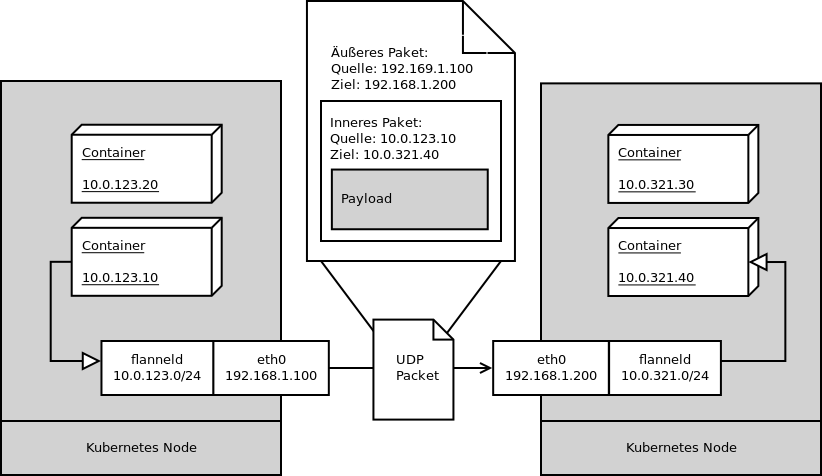
\includegraphics[width=1\textwidth]{flannel}
\caption{Vereinfachte Darstellung der flannel Logik. Angelehnt an Grafik aus
dem offiziellen flannel Repository \cite{flannel}}.
\end{figure}

\section{Dockerization}

Die einzelnen Komponenten müssen für den Betrieb in einem Kubernetes Cluster in
Docker Images umgewandelt werden, welche dann diese Prozesse als Container
ausführen.
Der Vorgang des Verpackens dieser Prozesse, auch \quotes{dockerize}
oder \quotes{containerize},
soll sich an folgenden Best-Practices orientieren:

\begin{description}
  \item[Images sollten möglichst klein sein.] Um später möglichst wenig Daten
  übertragen zu müssen und wenig Speicher auf dem Host Server einzunehmen,
  sollten die gebauten Docker Images möglichst klein bleiben.
  \item[Die Upstream-/Base-Images sollten vertrauenswürdig sein.]
  Sollte dieses Image unsicher oder fehlerhaft sein, oder im Laufe der Zeit
  werden, importiert man sich diese Probleme automatisch in sein eigenes Image.
  Es empfiehlt sich deshalb dringend, die Images aus den offiziellen Repositories
  zu verwenden \cite{DockerHub}.
  \item[Häufig wechselnde Layer sollten erst am Schluss gebaut werden.]
  Jeder Command in einem Dockerfile erzeugt einen neuen Layer im Docker-Image.
  Diese Layer können auf dem Build-Server gecached werden, sodass der nächste
  Build-Job diese dann nicht erneut bauen muss.
  Wenn sich ein Layer ändert, invalidiert er den Cache für alle folgenden Layer.
  Sofern sich der Layer, der sich oft ändert, relativ weit hinten befindet,
  beschleunigt das die Geschwindigkeit, in der diese Images gebaut werden können.
  Zudem werden gleiche Layer nicht für jedes Image neu abgespeichert, sondern
  werden von allen darauf aufbauenden Images verwendet. So spart dieses Vorgehen
  auch Speicherplatz ein.

\end{description}

Auf Grundlage dieser Punkte, werden nun im Root-Verzeichnis des jeweiligen
Git-Repositories, Dockerfiles angelegt,
welche die Anweisungen für das Zusammenbauen dieser Images enthalten.

\newcommand{\specialcell}[2][c]{%
  \begin{tabular}[#1]{@{}l@{}}#2\end{tabular}}

Am Beispiel des \emph{NodeJS} API Images soll verdeutlicht werden, wie diese Layer
genau aussehen werden.
\begin{flushleft}
\centering
\begin{tabular}{ | l | l | l | l | }
  \hline
  \# & Command & Anmerkung & Layergröße \\ \hline \hline
  1. & FROM node:6-alpine & \specialcell{Base-Image aus dem offiziellen \\ Docker-Hub Repository.}  & 17.2 MB \\ \hline
  2. & RUN mkdir -p /app/ & Erstellt Applikations Ordner & 91 B \\ \hline
  3. & WORKDIR /app/ & Setzt neues CWD & 0 B \\ \hline
  4. & COPY package.json . & Kopiert das Dependency File & 404 B \\ \hline
  5. & RUN npm install & \specialcell{Installiert alle externen \\ NodeJS Dependencies} & 16.6 MB \\ \hline
  6. & COPY . . & \specialcell{Kopiert alle restlichen \\ Applikations-Dateien} & 66 KB \\ \hline
  7. & CMD npm start & \specialcell{Setzt den Befehlt zum \\starten der Applikation} & 0 B \\ \hline
\end{tabular}
\captionof{table}
    [Layer des API Docker-Image]
    {Layer des API Docker-Image}
\end{flushleft}

Insgesamt kommt dieses Image auf eine Größe von 33.9 MB, was nicht zuletzt
an der Verwendung
des sehr kleinen \quotes{alpine} Base-Images liegt.

\section{Kubernetes Architektur}

Kubernetes besteht aus Master Node, mindestens einem Worker Node und
einem etcd Key/Value-Store, welcher für eine gewisse Fehlertoleranz aus mindestens
3 Servern bestehen sollte \cite{etcdclustersize}.
\begin{figure}[H]
\centering
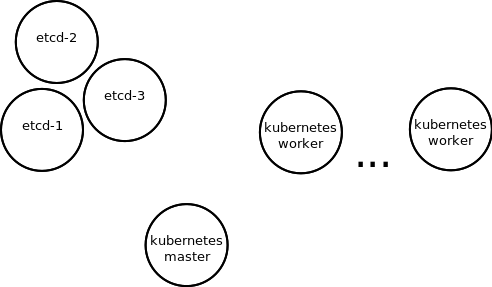
\includegraphics[width=0.5\textwidth]{kubernetes-komponenten}
\caption{Einfache Darstellung der benötigten Server}
\end{figure}

Die Worker Nodes haben in diesem Setup alle keine statischen IPs,
da sie je nach aktuellen Workload hoch und runter skaliert werden sollen.
Auf ihnen sollen beliebige Workloads laufen und ein Ausfall soll keine
schwerwiegenden
Folgen haben, denn ihre Workloads sind redundant und können von anderen Worker
Nodes übernommen werden.

Es gibt jedoch drei Arten von Workloads, für die eine statische \"offentliche IP-Adresse
und die Möglichkeit spezielle Workloads zu deployen unbedingt benötigt wird:
\begin{description}
  \item[Ingress Node:] Über diese Instanz soll der eingehende Traffic
  geroutet werden.
  Kubernetes stellt einen Ingress-Controller bereit, der Traffic entgegen
  nimmt und auf die internen
  Services des Clusters auf den Workern weiterleitet. Dieser
  Ingress-Controller
  ist ein Wrapper um \emph{Nginx} und rekonfiguriert \emph{Nginx}, sollte sich
  die Topographie der dahinter liegenden Backends ändern.
  \item[Admin Node:] Auf dieser Instanz werden die Tools installiert, die für
  Administratoren und Entwickler wichtig sind, um den reibungslosen Betrieb des
  Clusters und der darin befindlichen Applikationen zu prüfen.
  Auch hier läuft ein Ingress-Controller, der ausschließlich die Anfragen
  zu Admin-Frontends entgegen nimmt.
  Probleme auf dieser Instanz sollen die restlichen Instanzen nicht in
  Mitleidenschaft ziehen und sind deshalb ausgelagert.
  Durch diese zusätzliche Instanz kann außerdem auch verschleiert werden,
  unter welcher IP sich diese Tools verbergen, da der User in der Regel nur
  die IP der Ingress Node erfährt.
  Dies ist wichtig, da dieser Admin-Server für
  potentielle Angreifer ein besonders interessantes Angriffsziel bietet.
  \item[Testing Node:] Auf der Testing Node laufen die Staging- und
  Development-Environments. So können diese Environments im selben Cluster verwaltet werden,
  spielen aber im Betrieb der Production-Environment keine Rolle mehr, da sie
  auf dieser Node ausgelagert sind.
\end{description}

Mit dieser genaueren Spezifizierung der Worker Nodes,
sieht die Kubernetes-Architektur also folgendermaßen aus:
\begin{figure}[H]
\centering
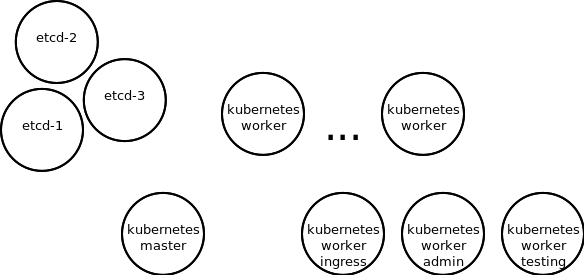
\includegraphics[width=0.5\textwidth]{kubernetes-komponenten-admin-ingress}
\caption{Einfache Darstellung der benötigten Server mit Ingress, Admin und Testing Node}
\end{figure}

\section{Netzwerk Architektur}

Damit die einzelnen Server-Instanzen auf AWS ausgeführt werden können, muss ein
Subnetz eingerichtet werden.
Über Terraform wird eine Virtual Private Cloud (VPC) geladen, in der Subnetze
und weitere Netzwerkkomponenten liegen.
Der IP-Adressraum dieses Subnetzes wird über einen
\quotes{Classless Inter-Domain Routing} (CIDR)-Block so gewählt,
dass es innerhalb eines privaten Adressraumes liegt \cite{CidrRfc}.
Das VPC, in dem die Subnetze liegen sollen, ist mit einem CIDR von
\code{10.0.0.0/16} groß genug,
um weitere Subnetze (zum Beispiel 255 Subnetze mit einer \emph{/24} Subnet-Mask)
anzulegen.
Das Subnetz, in das die Server-Instanzen migriert werden sollen, ist mit
\code{10.0.1.0/24} gewählt,
sodass damit 255 IP-Adressen besetzt werden können.
Einige dieser Adressen sind von AWS bereits belegt und für einige Server
des Kubernetes Setups werden statische private IP-Adressen benötigt
\cite{AwsVpc}.
Es macht also Sinn, ein konkretes Netzwerk-Layout zu bestimmen, welches in
folgender Tabelle zu sehen ist.

\begin{flushleft}
\centering
\begin{tabular}{ | l | l | l | }
  \hline
  IP-Adresse & Zweck \\ \hline \hline
  10.0.1.0 & Netzwerkadresse \\ \hline
  10.0.1.1 & AWS VPC-Router \\ \hline
  10.0.1.2 & AWS DNS-Server  \\ \hline
  10.0.1.3 & Reserviert von AWS für potentielle zukünftige Dienste \\ \hline
  10.0.1.4 & etcd Server 1 \\ \hline
  10.0.1.5 & etcd Server 2 \\ \hline
  10.0.1.6 & etcd Server 3 \\ \hline
  10.0.1.7 & Kubernetes Master Node \\ \hline
  10.0.1.8 & Reserviert für eine potentielle zweite Master Node \\ \hline
  10.0.1.9 & Kubernetes Ingress Node \\ \hline
  10.0.1.10 & Kubernetes Admin Node \\ \hline
  10.0.1.11 & Kubernetes Testing Node \\ \hline
  10.0.1.12-254 & Kubernetes Worker Nodes \\ \hline
  10.0.1.255 & Netzwerk-Broadcast \\ \hline
\end{tabular}
\captionof{table}
  [Netzwerk-Layout]
  {Netzwerk-Layout}
\end{flushleft}

Es bleiben also 243 IP-Adressen, welche in diesem Setup über DHCP dynamisch
an die Kubernetes Worker Nodes vergeben werden können.

Eine Alternative zu diesem Layout, ist, die Instanzen, die nicht unbedingt
aus dem Internet erreichbar sein müssen (etcd und Worker Nodes), in ein privates
Subnetz zu starten,
das nur aus dem \"offentlichen Subnetz, nicht aber aus dem Internet, erreichbar
ist.
Dementsprechend bekommen diese Instanzen dann nur eine private IP-Adresse und
keine
\"offentliche IP-Adresse.

Ein Grund, warum auf das private Subnetz an dieser Stelle verzichtet wird,
ist, dass die Instanzen im privaten Subnetz eine NAT-Instanz benötigen würden,
um sich mit dem Internet zu verbinden.
Die NAT Instanz ist dann ein \emph{Single Point of Failure} und die
Netzwerk-Architektur
wird komplizierter und schwerer zu warten, da man sich auf die privaten
Instanzen dann nur noch
mittels eines Bastion-Servers verbinden kann.
Außerdem würde eine weitere Instanz auch höhere Kosten verursachen und zu
höherem Vendor Lock-in führen.
Die Hosts des Clusters, die sich über das NAT ins Internet verbinden,
haben dann nach außen alle dieselbe \"offentliche IP-Adresse.
So kann es passieren, dass externe Services, Requests dieser Server
mittels Rate-Limiting blocken, wenn beispielsweise alle Hosts gleichzeitig ein
Docker Image von einem externen Provider herunterladen.

Der Vorteil, dass ein privates Subnetz stärker nach außen hin abgeschirmt ist,
wiegt die Nachteile in diesem Use Case nicht auf.
Die geringere Abschirmung kann mit entsprechender Firewall-Konfiguration und
Absicherung der nach innen gerichteten Schnittstellen begegnet werden.

\section{Instanz Typen}

\subsection{etcd Instanzen}
Während CPU und Memory eher weniger im Fokus liegen,
ist es wichtig, dass eine möglichst schnelle Festplatte vorhanden ist
\cite{etcdhardware}.
Aus diesem Grund sind die \code{t2.nano}-Instanzen besonders gut geeignet.
Sie kosten pro Instanz nur \$ 4.75 pro Monat und werden standardmäßig mit einer
8GB SSD Festplatte mit 65.000 IOPS bereit gestellt \cite{AwsEbs}.

\subsection{Master Node}
Die Kubernetes Master Node braucht zwar nicht besonders viele Hardware-Ressourcen,
da das Cluster-Management nur relativ wenige Ressourcen verbraucht,
solange es sich um ein kleineres Cluster handelt. Da aber die Master Node eine
kritische Instanz für den Betrieb des Clusters ist, und gute Hardware den
Start und Neustart dieser Instanz beschleunigt,
soll an diesem Server nicht gespart werden. Die \code{t2.medium}-Instanzen mit
4 GB Memory und 2 vCPUs bis 3,3 GHz, bieten dafür ausreichende Leistung.

\subsection{Worker Nodes}
Worker Nodes sind die Server, die unter Last in ihrer Anzahl hoch und runter
gesetzt werden sollen,
um die Leistungsfähigkeit des Clusters entsprechend zu skalieren.
Um eine möglichst granulare Skalierung zu erlauben, sollten diese
Instanzgrößen nicht zu groß gewählt sein.
Die \code{t2.small}-Instanzen stellen eine vCPU mit bis zu 3,3 GHz bereit
\cite{Awst2}.
Zudem stehen 2 GB Memory und 8 GB SSD Festplattenspeicher bereit.

\subsection{Ingress Node}
Die Ingress Instanz ist der Entrypoint für die User und sollte deshalb
nicht zu klein gewählt sein. Für den Anfang reicht hier eine
\code{t2.medium}-Instanz.

\subsection{Admin Node}
Auf dieser Node laufen zahlreiche Prozesse f\"ur die Administration des Clusters.
Um diese Prozesse mit ausreichender Leistung versorgen zu k\"onnen, empfiehlt sich
eine \code{t2.medium}-Instanz.

\subsection{Testing Node}
Für die Testing Node reicht wieder eine \code{t2.small}-Instanz.
Bei Bedarf kann diese jederzeit upgedatet werden.



\section{Installation des Kubernetes Clusters}

\subsection{Generierung der TLS Assets}
Um die Kommunikation zwischen den Worker Nodes, dem eigenen Laptop und der
Master Node abzusichern,
müssen Zertifikate und Keys generiert werden. Mit dem \code{local-exec} Modul kann mit
Terraform ein lokales Script ausgeführt werden.
Zuerst wird eine Certificate-Authority (CA) erstellt, aus der die weiteren
Zertifikate und Keys entstehen werden.
Die Client-Keys und Zertifikate für \code{kubectl} und die Master Node können
schon im Vorfeld
auf dem lokalen Rechner erstellt werden.
Die Schwierigkeit, die sich beim Erstellen der Worker Node Zertifikate und Keys
ergibt,
ist, dass im Vorfeld nicht bekannt ist, welche private IP der jeweiligen Instanz
zugeordnet wird.
Diese Information ist aber wichtig, weil das Zertifikat beglaubigen
soll, um welchen
Server (im Sinne der privaten IP) es sich genau handelt.
Die Worker Nodes müssen zwangsläufig ausschließlich über die \emph{Cloud-Config}
konfigurierbar sein,
da das die einzige Option ist, die bei Launch Configuration von
\emph{Auto Scaling Groups} zur Verfügung steht.
Hierauf wird in einem späteren Abschnitt genauer eingegangen.

Es gibt nun zwei Möglichkeiten, um dieses Problem zu lösen:
\begin{itemize}
  \item Die Zertifikate und Keys werden für alle potentiell möglichen 243
  Worker Node
  IP-Adressen erstellt,
  diese müssen dann \textbf{alle} per \emph{Cloud-Config} auf \textbf{jede} Worker Node
  übertragen werden, wo die Worker Node sich,
  je nach tats\"achlich zugewiesener IP-Adresse, die richtige raussucht.
  \item Die CA und der dazugehörige CA-Key werden per \emph{Cloud-Config} auf den
  Server übertragen,
  die Node erstellt sich selbst das Zertifikat und den Key und löscht danach
  wieder CA und CA-Key,
  sodass diese für einen potentieller Angreifer nicht mehr zu finden sind.
\end{itemize}

Beide Lösungen sind nicht zu 100 Prozent sauber und gewissermaßen \quotes{hacky}.
Da die \emph{Cloud-Config} nicht größer als 16384 Bytes \cite{AwsCloudConfig} werden
darf,
ist an dieser Stelle nur die zweite Lösung praktikabel.

\subsection{etcd Konfiguration}
Wie bereits erörtert, wird \emph{etcd} in einem 3-Server-Cluster gestartet.
Bei 3 Servern kann ein Server ausfallen, ohne dass das Cluster komplett ausfällt,
denn mit 2 übrigen Servern, kann weiterhin eine Leader-election stattfinden und
das Quorum bleibt erhalten \cite{etcdclustersize}.

\emph{etcd} stellt einen kostenlosen Service Discovery Server zur Verfügung.
Die einzelnen Instanzen verbinden sich mit diesem und geben die private
IP-Adresse bekannt, unter der sie im Subnetz zu finden sind. Wenn sich alle
Cluster Members auf diesem Weg gefunden haben, ist das etcd-Cluster
betriebsbereit.

Da aber in diesem Fall die privaten IP-Adressen bereits im Vorfeld bekannt sind,
weil sie bereits
durch die Netzwerk-Architektur festgelegt wurden, und, weil keine Details
über den internen Aufbau des Cluster nach außen preisgegeben werden sollen,
sind die IP-Adressen in diesem Fall besser \quotes{hardcoded} zu implementieren.
Dadurch erübrigt sich die Abhänigigkeit zur Service Discovery für diesen Zweck.

Per \emph{Cloud-Config} wird deshalb diese Konfiguration gesetzt:

\begin{lstlisting}[language=Python,numbers=none]
etcd2:
  name: infra${counter}
  advertise-client-urls: http://$private_ipv4:2379
  listen-client-urls: http://0.0.0.0:2379
  initial-advertise-peer-urls: http://$private_ipv4:2380
  listen-peer-urls: http://$private_ipv4:2380
  initial-cluster-token: etcd-cluster-1
  initial-cluster: "infra0=http://10.0.1.4:2380,infra1=http://10.0.1.5:2380,infra2=http://10.0.1.6:2380"
  initial-cluster-state: "new"\end{lstlisting}

Die Instanzen, die auf dieses etcd-Cluster zugreifen wollen, sollen nicht als
weitere Member in dieses Cluster angemeldet werden, sondern nur eine
Proxy-Verbindung
zu diesem aufbauen \cite{CoreOSCluster}.
So ist dem \emph{Seperation of Concerns}-Prinzip Folge geleistet und potentieller
Overhead
durch Synchronisierung einer großen Anzahl von Nodes kann vermieden werden.
Die Konfiguration wird über die \emph{Cloud-Config} folgendermaßen vorgenommen:

\begin{lstlisting}[language=Python,numbers=none]
etcd2:
  proxy: on
  listen-client-urls: http://127.0.0.1:2379
  initial-cluster: "infra0=http://10.0.1.4:2380,infra1=http://10.0.1.5:2380,infra2=http://10.0.1.6:2380"\end{lstlisting}

Jede Instanz ist nun entweder \emph{etcd}-Member oder als Proxy mit diesen
verbunden.
In der folgenden Graphik ist dies graphisch verdeutlicht.

\begin{figure}[H]
\centering
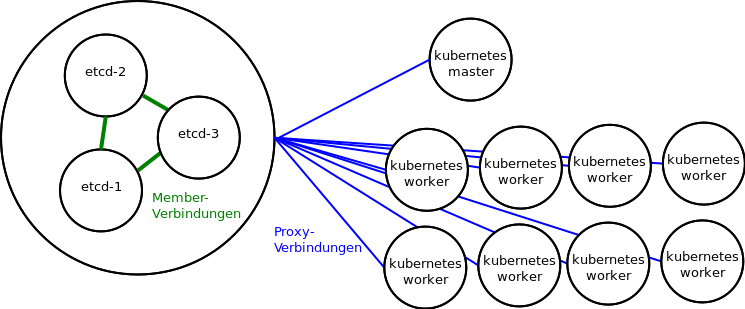
\includegraphics[width=1\textwidth]{etcd}
\caption{Member- und Proxy-Verbindungen des etcd Setups}
\end{figure}

\subsection{kubelet Konfiguration}
Auf CoreOS ist ein Script vorinstalliert, welches das \emph{kubelet} herunterlädt und
an dieses diverse Parameter durchreicht.
Das automatische Starten dieses Scriptes wird durch \emph{systemd}-Units ausgelöst,
welche über \emph{Unit files} in der \emph{Cloud-Config} auf den Server geladen werden.
Sobald das \emph{kubelet} gestartet wurde, startet dieses wiederum weitere Komponenten,
deren Kubernetes-Manifeste in \code{/etc/kubernetes/manifests} auch
mittels der \emph{Cloud-Config} abgelegt wurden.
Diese Manifeste starten nun die einzelnen Container, welche auf Master Node
und Worker Nodes benötigt werden.
Im Einzelnen sind das auf der Master Node folgende Container:

\begin{description}
  \item[kube-apiserver] Die zentrale Stelle, um mit dem Kubernetes-Cluster zu
  interagieren.
  Es bietet eine REST-API an, welche auf dem Host über das
  \code{localhost}-Netzwerk-Interface auf Port 8080 angesprochen werden kann.
  Nach außen hin steht eine HTTPS Schnittstelle auf Port 443 zur Verfügung.
  Die bereits erstellten Zertifikate und Keys,
  welche mittels \emph{Cloud-Config} in \code{/etc/kubernetes/ssl} abgelegt wurden,
  sichern diesen Port.
  \item[kube-controller-manager] Diese Komponente ist dafür zuständig,
  den gewünschten Zustand, in dem sich das Cluster befinden soll,
  mit dem tatsächlichen zu vergleichen. Je nachdem, welche Veränderung notwendig
  ist, um das Cluster in den gewünschten Zustand zu bekommen, schickt diese
  Komponente
  Aufträge an den \emph{kube-scheduler}.
  \item[kube-scheduler] Der Scheduler ist dafür zuständig auf den einzelnen Nodes,
  egal ob Worker oder Master, Workloads zu platzieren. Dafür benutzt der Scheduler
  auch Daten über die Ressourcen der Server, die Availability und
  weitere Bedingungen \cite{k8sscheduler}.
  \item[kube-proxy] Läuft als \emph{DaemonSet} auf allen Nodes und ist dafür
  zuständig TCP und UDP Traffic an die
  jeweiligen Services auf dem Host weiterzuleiten. Jeder Pod hat in
  Kubernetes auch seine eigene IP-Adresse
  im \emph{flannel} Network Overlay, an die Traffic weitergeleitet wird.
\end{description}

Auf den Worker Nodes wird vom \emph{kubelet} nur der \emph{kube-proxy} gestartet.

In folgender Grafik ist die initiale Bootstrap-Logik verdeutlicht.

\begin{figure}[H]
\centering
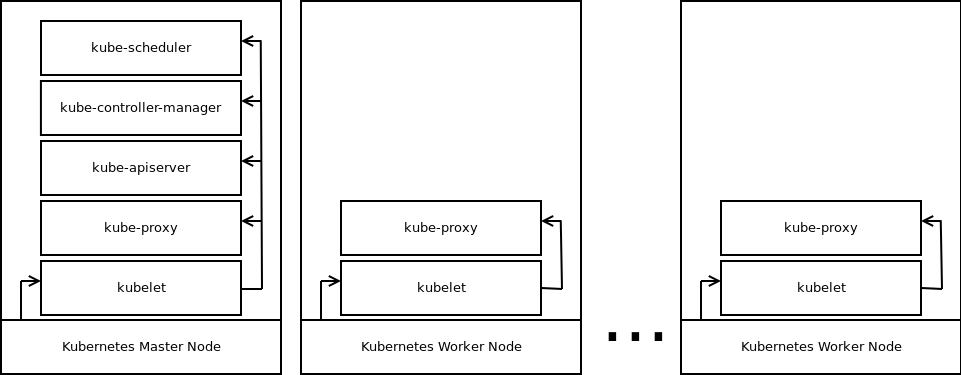
\includegraphics[width=1\textwidth]{server-containers-initial}
\caption{Bootstrapping der Instanzen}
\end{figure}

\subsection{locksmith Konfiguration}

Über \emph{locksmith} wird eine Update-Strategie bestimmt, mit der
CoreOS automatisch Updates aufspielen soll.
Wie bereits beschrieben, lädt CoreOS neue Builds aus den Release Channels, und
speichert diese in einer separaten Partition. Um von der alten auf die neue
Partition zu wechseln,
muss das Betriebssystem neugestartet werden.
Mit locksmith wird festgelegt, wann das passieren darf.

In dieser Umsetzung gibt es mehrere Host-Gruppen, die
nie komplett ausfallen dürfen. Sollten zum Beispiel plötzlich alle Worker Nodes
rebooten,
wäre die API, Website und andere Komponenten nicht mehr erreichbar.
Aus diesem Grund wird hier ein etcd-lock benutzt. Im Wesentlichen stellt dieses
\emph{etcd-lock} sicher, dass immer nur eine Maschine neugestartet wird.
So setzt die Instanz, die neustarten soll, ein Key/Value-Pair
mit einer Referenz zu sich selbst und der Gruppe in der sie gerade neustartet.
Erst wenn diese Instanz nach dem Neustart, dieses Key/Value-Pair wieder
freigibt, darf
die nächste Instanz aus dieser Gruppe neustarten.
So rebooten sich die Instanzen nach und nach von selbst.

Desweiteren kann ein Zeitrahmen festgelegt werden, in dem solche Updates überhaupt
stattfinden dürfen. In diesem Fall empfiehlt es sich, einen Zeitpunkt zu
wählen,
indem im Zweifel manuell eingegriffen werden kann und das Cluster
nicht gerade die höchste Last zu verarbeiten hat.
Die exemplarische Entscheidung ist hier auf Donnerstag ab 16:00 UTC für einen
Zeitraum von einer Stunde gefallen,
wie man an dieser \emph{Cloud-Config} für alle Worker Nodes sieht:

\begin{lstlisting}[language=Python,numbers=none]
update:
  reboot-strategy: etcd-lock
  group : "worker"
locksmith:
  window-start: Thu 16:00
  window-length: 1h
  endpoint: http://127.0.0.1:2379\end{lstlisting}

\subsection{flannel Konfiguration}
Es reicht für die Konfiguration, den etcd-Endpoint anzugeben und die Information
auf welchem Netzwerk-Interface es sich anmelden soll.
\begin{lstlisting}[language=Python,numbers=none]
flannel:
  interface: $private_ipv4
  etcd_endpoints: http://127.0.0.1:2379\end{lstlisting}

Docker muss nun so eingestellt werden, dass es erst startet, nachdem flannel
gestartet wurde. Für diesen Zweck wurde diese Abhängigkeit per
\emph{systemd} Drop-in der Docker Unit deklariert.

\begin{lstlisting}[language=Python,numbers=none]
- name: docker.service
  command: start
  drop-ins:
    - name: 40-flannel.conf
      content: |
        [Unit]
        Requires=flanneld.service
        After=flanneld.service
        ...\end{lstlisting}

\section{Firewall}

\subsection{Internet}

Wie bereits bezüglich des privaten Subnetzes erwähnt, liegen alle Instanzen in
einem \emph{Public Subnet}, in dem Sie mit ihrer IP-Adresse direkt aus dem Internet erreicht werden können.
Umso wichtiger, besonders genau darauf zu achten, dass alle Hosts gut
mit einer Firewall geschützt sind.

Ohne Firewall-Regeln stehen eine Reihe unnötiger Ports offen,
was man an folgendem \code{nmap} Auszug sehen kann:

\begin{lstlisting}[language=Python,numbers=none]
Host is up (0.040s latency).
Not shown: 65523 closed ports
PORT      STATE    SERVICE
22/tcp    open     ssh
135/tcp   filtered msrpc
137/tcp   filtered netbios-ns
138/tcp   filtered netbios-dgm
139/tcp   filtered netbios-ssn
443/tcp   open     https
445/tcp   filtered microsoft-ds
4194/tcp  open     unknown
10250/tcp open     unknown
10251/tcp open     unknown
10252/tcp open     unknown
10255/tcp open     unknown\end{lstlisting}

Von all diesen Ports wird auf der Master Node aber nur Port \code{443} für
den API Server und Port \code{22} für die \emph{Secure Shell} benötigt. Mit der folgenden
Security Group-Konfiguration in Terraform werden alle anderen Ports geschlossen.

\begin{lstlisting}[language=Python,numbers=none]
ingress {
  from_port   = 22
  to_port     = 22
  protocol    = "tcp"
  cidr_blocks = ["0.0.0.0/0"]
}

ingress {
  from_port   = 443
  to_port     = 443
  protocol    = "tcp"
  cidr_blocks = ["0.0.0.0/0"]
}\end{lstlisting}

\code{nmap} gibt dann folgendes Ergebnis zurück.

\begin{lstlisting}[language=Python,numbers=none]
Host is up (0.060s latency).
Not shown: 65533 filtered ports
PORT    STATE SERVICE
22/tcp  open  ssh
443/tcp open  https\end{lstlisting}

Auf gleiche Weise müssen auch alle anderen Hosts konfiguriert werden, sodass
am Schluß nur noch die tats\"achlich n\"otigen Ports offen sind.
Welche das sind, ist in folgender Grafik verdeutlicht:

\begin{flushleft}
\centering
\begin{tabular}{ | l | l | l | l | }
  \hline
  Instanz & Port & L3 Protokoll & Zweck \\ \hline \hline
  Alle & 22 & TCP & SSH Zugang \\ \hline
  Master & 443 & TCP & API-Server  \\ \hline
  Worker Ingress & 80 + 443 & TCP & Nginx Ingress \\ \hline
  Worker Admin & 80 + 443 & TCP & Nginx Ingress \\ \hline
  Worker Testing & 80 + 443 & TCP & Nginx Ingress \\ \hline
  Worker Admin & 5000 & TCP & Docker Registry \\ \hline
\end{tabular}
\captionof{table}
    [Firewall-Regeln in das Internet]
    {Firewall-Regeln in das Internet}
\end{flushleft}

Man beachte, dass die \emph{etcd} Hosts, bis auf Port 22, komplett abgeschirmt sind.
Auch die normalen Worker Nodes brauchen nur Port 22, selbst wenn auf ihnen
Web-Backends laufen, denn die
Stelle an der diese Verbindungen angenommen werden, ist die Ingress Instanz.
Diese leitet die Anfrage über das flannel \emph{vxlan} im Subnetz
weiter an die Instanzen, auf denen diese Pods laufen.

\subsection{Privates Subnetz}

Neben der Firewall-Konfiguration, die vor Zugriffen aus dem Internet abschirmt,
empfiehlt es sich, auch die Ports der Instanzen ins eigene Subnetz zu sperren,
sollten diese nicht unbedingt notwendig sein. In folgender Tabelle sind
die Ports aufgeführt, die offen bleiben müssen.

\begin{flushleft}
\centering
\begin{tabular}{ | l | l | l | l | l | }
  \hline
  Instanz & Port & L3 Protokoll & Zweck \\ \hline \hline
  etcd & 2379 & TCP & etcd Client  \\ \hline
  etcd & 2380 & TCP & etcd Peer \\ \hline
  Master & 443 & TCP & API-Server \\ \hline
  Master und Worker & 8472 & UDP & flannel vxlan  \\ \hline
  Master und Worker & 10250 & tcp & kubelet \\ \hline
  Master und Worker & 10255 & tcp & heapster \\ \hline
\end{tabular}
\captionof{table}
    [Firewall-Regeln in das Subnetz]
    {Firewall-Regeln in das Subnetz}
\end{flushleft}

\section{Auto Scaling Group}

\emph{Auto Scaling Groups} ist ein AWS Feature, welches erlaubt, Gruppen von
Instanzen zu überwachen und auf Grundlage bestimmter Metriken weitere
Instanzen zu starten oder aktive Instanzen zu terminieren.
In folgendem Snippet ist die Terraform-Konfiguration für diese
\emph{Auto Scaling Group} zu sehen.

\begin{lstlisting}[language=Python,numbers=none]
resource "aws_autoscaling_group" "worker" {
  name = "k8s-aws_autoscaling_group"

  desired_capacity          = "2"
  health_check_grace_period = 60
  health_check_type         = "EC2"
  force_delete              = true
  launch_configuration      = "${ aws_launch_configuration.worker.name }"
  max_size                  = "8"
  min_size                  = "2"
  vpc_zone_identifier       = ["${aws_subnet.k8s-public.id}"]

  tag {
    key                 = "Name"
    value               = "k8s-worker"
    propagate_at_launch = true
  }
}\end{lstlisting}

Um diese \emph{Auto Scaling Group} anzusteuern, gibt es mehrere
Möglichkeiten. Diese
sollen beleuchtet werden, sobald die Art der Workloads genauer erörtert wurde.
An dieser Stelle sei nur erwähnt, dass diese \emph{Auto Scaling Group} eine
Schnittstelle
bietet, um Instanzen mit einer gewissen \emph{Launch Configuration} zu starten oder
zu terminieren.
Initial startet sie an dieser Stelle die 2 Instanzen, die unter
\code{desired\_capacity}
definiert wurden.

\section{Start der Terraform Konfiguration}
Die beschriebenen Konfigurationen werden per Terraform deployed.
Die Reihenfolge der Aktivierungen hängt von den Abhängigkeiten
der einzelnen Module ab.
Terraform erstellt dazu intern einen Abhängigkeits-Graphen. Zum Zwecke
der Verständlichkeit
sollen an dieser Stelle grob die Schritte in chronologischer
Reihenfolge aufgelistet sein:

\begin{enumerate}
  \item Generiere die TLS Assets auf dem lokalen Rechner
  \item Erstelle ein VPC mit Subnetz und Internet-Gateway
  \item Starte die 3 etcd Instanzen
  \item Starte die Kubernetes Master Node
  \item Starte die Kubernetes Worker Nodes (Auto Scaling Group, Admin, Testing
  und Ingress)
  \item Worker Nodes warten bis der Kubernetes Master erreichbar wird und starten
  dann jeweils das eigene Kubelet Setup
  \item Security Groups werden auf die Instanzen angewandt
  \item DNS A-Records in Route53 werden mit der IP der
  jeweiligen Instanz konfiguriert
\end{enumerate}

Danach dauert es im Durchschnitt 8 Minuten, bis die Instanzen hochgefahren sind
und die \emph{kubelets}, sowie alle
weiteren Basis-Komponenten heruntergeladen und gestartet wurden. Außerdem müssen
die DNS-Einträge noch verbreitet werden, was unterschiedlich lange dauern kann.
Sobald \code{kubectl get nodes} alle Nodes mit Status \quotes{Ready} anzeigt,
ist das Cluster betriebsbereit.

\begin{lstlisting}[language=Python,numbers=none]
$ kubectl get nodes
NAME            STATUS                     AGE
ip-10-0-1-7     Ready,SchedulingDisabled   2m
ip-10-0-1-9     Ready                      1m
ip-10-0-1-10    Ready                      54s
ip-10-0-1-11    Ready                      50s
ip-10-0-1-123   Ready                      58m
ip-10-0-1-196   Ready                      1m\end{lstlisting}

\begin{tcolorbox}
  Hinweis: An dieser Stelle ist Kubernetes betriebsbereit.
  In den folgenden Abschnitten wird es darum gehen, die Addons und die
  Domain-Logik in diesem Cluster mittels Manifest-Dateien aufzusetzen.
\end{tcolorbox}

\section{Namespaces}

Namespaces stellen eine Form der Isolierung unterschiedlicher Workloads dar.
So kann verhindert werden, dass ein Pod, der beispielsweise als Test-Frontend läuft,
auf Pods oder Services zugreift, die Administrations-Aspekte des Clusters regeln.
Aus diesem Grund werden alle Pods in unterschiedliche Namespaces deployed, welche
sich wie folgt darstellen:

\begin{description}
  \item[kube-system:]
  Hier sollen alle Pods laufen, welche sich mit der Administration des
  Clusters selbst befassen.
  \item[Production:]
  In diesem Namespace werden Pods deployed, die die Domain-Logik für die echten
  User behandeln.
  \item[Testing:]
  Hier werden die Staging- und die Development-Environment abgebildet. Warum
  diese nicht jeweils ihren eigenen Namespace haben, wird im Abschnitt zu den
  Ingress-Controllern genauer erörtert.
\end{description}

Erst wenn diese Namespaces erzeugt wurden, lassen sich auch Komponenten in diesen
unterbringen.

In diesem Szenario ergibt sich durch die Namespaces auch eine lose Zuordnung auf
die unterschiedlichen Nodes, welche in einem späteren Abschnitt genauer
beleuchtet werden.

\section{Cluster-Addons}

\subsection{DNS}
Mit dem \emph{kube-dns} Pod und Service können die einzelnen Ressourcen, die
auf dem Cluster eine IP im Overlay Network zugewiesen bekommen haben, direkt über
Hostnamen angesprochen werden. Dies macht die Kommunikation der Services einfacher,
denn IPs können sich ändern, der DNS-Eintrag wird aber immer auf die richtige
IP-Adresse zeigen.
Beim Initialisieren der Worker Kubelets, musste die Cluster-IP des
DNS-Servers spezifiziert
werden:
\begin{lstlisting}[language=Python,numbers=none]
ExecStart=/usr/lib/coreos/kubelet-wrapper
...
--cluster-dns=10.3.0.10\end{lstlisting}
Unter dieser Adresse wird nun der \emph{kube-dns} Pod gestartet. Jetzt können über
diesen Pod
die IP-Adressen für interne und externe Hostnamen angefragt werden, wie in
diesem Beispiel, welches auf einem
anderen Pod im Cluster ausgeführt wird, zu sehen:
\begin{lstlisting}[language=Python,numbers=none]
$ nslookup kubernetes
Server:    10.3.0.10
Address 1: 10.3.0.10 kube-dns.kube-system.svc.cluster.local

Name:      kubernetes
Address 1: 10.3.0.1 kubernetes.default.svc.cluster.local\end{lstlisting}
Wenn also \emph{kube-dns} nach der Adresse des API-Servers
(Hostname \quotes{kubernetes}) gefragt wird,
antwortet \emph{kube-dns} richtig mit \code{10.3.0.1}.

\subsection{Dashboard}
Oft ist das Analysieren und das Eingreifen im Cluster über die Console
relativ mühsam.
Um dies einfacher zu machen, stellt Kubernetes ein Dashboard bereit,
welches auch als Pod im Cluster deployed wird.

\begin{figure}[H]
\centering
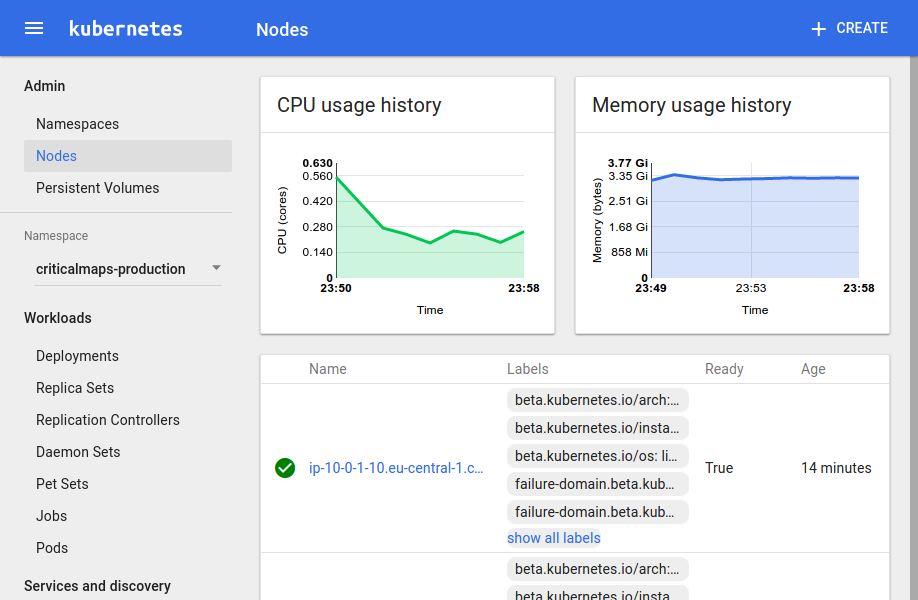
\includegraphics[width=1\textwidth]{dashboard}
\caption{Screenshot des Kubernetes Dashboards}
\end{figure}

Der Zugriff auf das Dashboard läuft über einen Proxy, der eine Verbindung
in das Kubernetes-Cluster tunnelt.
Gestartet wird dieser Proxy mit \code{kubectl proxy}.
\begin{lstlisting}[language=Python,numbers=none]
$ kubectl proxy
Starting to serve on 127.0.0.1:8001\end{lstlisting}

Auf den lokalen Rechner kann es dann unter:
\\
\code{http://localhost:8001/api/v1/proxy/namespaces/kube-system} \\
\code{/services/kubernetes-dashboard/\#/node?namespace=default}

aufgerufen werden. Es muss, dank Proxy, nicht immer ein Endpoint
nach außen freigegeben werden. In diesem Fall ist der Proxy der sicherste Weg,
das Dashboard den Cluster-Admins zur Verfügung zu stellen. Für andere Zielgruppen,
die keinen \code{kubectl} Zugriff haben, müssen jedoch
weiterhin Endpoints nach außen exponiert werden.

\begin{tcolorbox}
  Hinweis: Mit \emph{kube-dns} und dem Dashboard sind die zwei Pods installiert,
  die als offizielles Kubernetes-Addon angeboten werden
  und zur Standard-Ausstattung der meisten Kubernetes-Cluster zählen, da
  sie elementare Funktionalität bereitstellen.
  Zwingend
  notwendig sind sie aber nicht.
  In folgenden Abschnitten sollen weitere Pods installiert werden, welche
  nicht mehr zu dieser Standardausstattung gezählt werden.
\end{tcolorbox}

\section{Admin-Addons}

Mit Admin-Addons sind die Tools gemeint, die Admins und gegebenenfalls auch
Entwicklern, Informationen über das Cluster und die darin laufenden
Applikationen geben.
Ganz konkret geht es hier um Logging, Monitoring und Alerting. Für diesen
Zweck werden drei verschiedene Tools installiert.

\begin{tcolorbox}
Anmerkung: Elasticsearch, die Firma hinter dem ELK-Stack, will diese drei Dinge
unter ihrem Stack bündeln und bietet dafür ein erweitertes Paket an Open Source
Software an. Bei dem Versuch diese Software auf diesen Anwendungsfall anzuwenden,
haben sich jedoch eine Reihe Probleme aufgetan, die voraussichtlich mit der
Weiterentwicklung
dieser Software in naher Zukunft gelöst werden. Aus diesem Grund und aufgrund des
\emph{Separation of Concerns}-Patterns, wurden jeweils eigentändige
Komponenten gewählt.
\end{tcolorbox}

\subsection{Logging}
Die Container, die in das Cluster deployed werden, loggen auf
\code{stdout} und \code{stderr}.
Um diese Logs ohne weitere Hilfsmittel einsehen zu können, kann kubectl
folgendermaßen benutzt werden:
\begin{lstlisting}[language=Python,numbers=none]
$ kubectl logs container_name pod_name\end{lstlisting}
Theoretisch kann auch SSH benutzt werden, um auf die Node zu kommen, auf der der
Container läuft, um dort direkt in die Logdateien zu sehen, oder um
\begin{lstlisting}[language=Python,numbers=none]
$ docker logs container_name\end{lstlisting}
zu benutzen. Dies wäre aber noch komplizierter, da auch im Vorfeld bekannt
sein
muss, auf welche Node dieser Container vom \emph{kube-scheduler} deployed wurde.

Es ist also wichtig, eine einfachere Option bereitzustellen, um auf diese
Logs zugreifen zu können.
Mit dem ELK-Stack können diese Logs eingelesen, abgespeichert und aufbereitet
dargestellt werden.
Der ELK-Stack besteht aus \textbf{E}lasticsearch \cite{elasticsearch},
\textbf{K}ibana \cite{kibana} und
\textbf{L}ogstash \cite{logstash}.

\begin{description}
  \item[Logstash/Fluentd:]
  Logstash ist Software, die Daten, wie Logs einliest, gegebenenfalls aufbereitet und
  schließlich zum weiteren Gebrauch an Elasticsearch oder eine weitere Logstash
  Einheit schickt.
  Tatsächlich soll aber in dieser Arbeit das eigentliche Logstash nicht
  verwendet werden,
  sondern nur das Format mit diesen Daten abgespeichert werden.
  \emph{Fluentd} \cite{fluentd} hat sich als einfacher in der Konfiguration herausgestellt und
  vereinnahmt auch weniger Memory auf der Maschine.
  Der \emph{Fluentd}-Pod, muss auf jeder Node vorhanden sein. Aus diesem Grund wird
  \emph{Fluentd}
  als \emph{DaemonSet} installiert. Bei einem \emph{DaemonSet} wird vom \emph{kube-scheduler}
  \textbf{ein} Pod dieser Konfiguration auf \textbf{jeder} Node platziert.
  Auf der jeweiligen
  Node, wird
  der Ordner, in dem Docker die Logs ablegt, gemapped:
  \begin{lstlisting}[language=Python,numbers=none]
  volumes:
  - name: varlibdockercontainers
    hostPath:
      path: /var/lib/docker/containers  \end{lstlisting}
  und in den Container gemountet:
  \begin{lstlisting}[language=Python,numbers=none]
  volumeMounts:
  - name: varlibdockercontainers
  mountPath: /var/lib/docker/containers
  readOnly: true  \end{lstlisting}
  \emph{Fluentd} hat dann Zugriff auf diese Logdateien und wird
  mit folgender Konfiguration so eingestellt, dass es allen Logfiles
  mittels \code{tail} folgt und neue Logzeilen entgegen nimmt.
  \begin{lstlisting}[language=Python,numbers=none]
  <source>
    @type tail
    read_from_head true
    path /var/lib/docker/containers/*/*-json.log
    pos_file /var/log/fluentd-docker.pos
    time_format %Y-%m-%dT%H:%M:%S
    tag docker.*
    format json
  </source>  \end{lstlisting}

  Die Weitergabe im Logstash-Format an Elasticsearch erfolgt dann über
  diese Konfiguration:
  \begin{lstlisting}[language=Python,numbers=none]
  <match *.**>
    @type elasticsearch
    logstash_format true
    host elasticsearch-logging
    port 9200
  </match>  \end{lstlisting}
  Wie man sieht, kann anstatt der Elasticsearch IP-Adresse hier der
  Hostname eingetragen werden, da \emph{kube-dns} diesen Hostnamen in die IP des
  Elasticsearch-Service
  auflösen wird.
  Zudem ist anzumerken, dass mit \emph{Fluentd} die Logs zwar in die
  Elasticsearch-Datenbank kopiert werden,
  aber eben nicht von der Node gelöscht werden. Um zu verhindern,
  dass exzessives Logging irgendwann
  die Festplatte überflutet, sollte der Docker Logging-Driver so eingestellt
  werden, dass er nach 10 Megabyte anfängt
  die Log-Dateien zu rotieren:
  \begin{lstlisting}[language=Python,numbers=none,breaklines=true]
  Environment="DOCKER_OPTS=--log-opt max-size=10m"\end{lstlisting}

  \item[Elasticsearch:]
  Elasticsearch ist die Datenbank, welche die Daten hält, die von \emph{Fluentd}
  gesammelt werden.
  Speziell für diese Text-Daten ist Elasticsearch besonders gut geeignet und kann
  mit großen Mengen dieser Daten umgehen \cite{elasticsearch}.
  Theoretisch kann Elasticsearch im \quotes{cluster-mode} laufen, in dem
  mit Shards- und Replica-Pods für höhere Ausfallsicherheit und Performance
  gesorgt wird.
  Da es sich hier aber um ein internes Tool handelt und die
  Logging-Anforderungen überschaubar sind,
  wird Elasticsearch
  nur als einzelner Pod
  betrieben.

  \item[Kibana:]
  Kibana ist das Web-Frontend, welches die Daten aus Elasticsearch
  grafisch aufbereitet anzeigt. Neben dem einfachen Anzeigen der
  Logs auf Grundlage
  diverser Filter,
  lassen sich auch komplexe Dashboards anlegen.
  \begin{figure}[H]
  \centering
  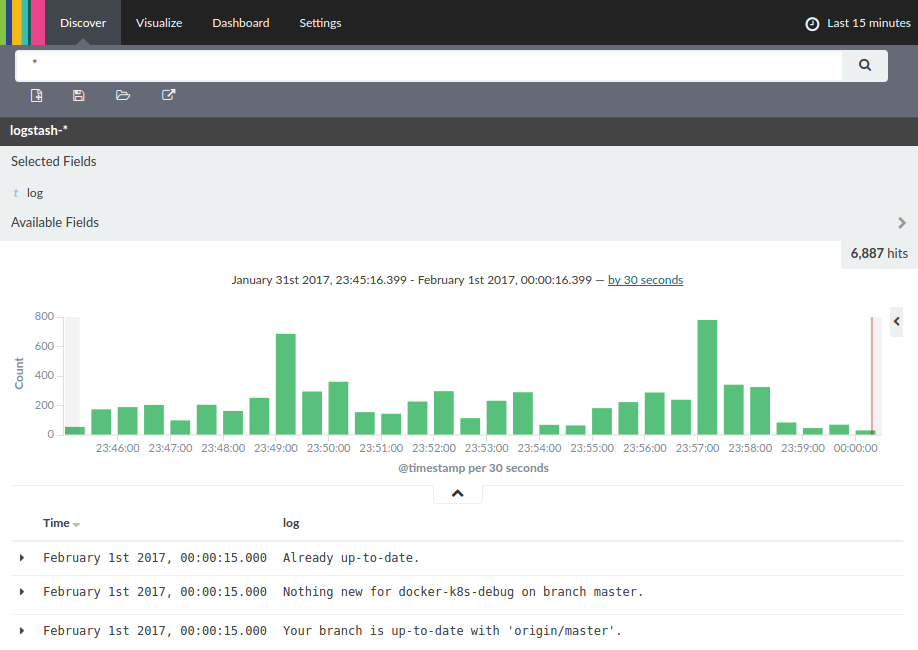
\includegraphics[width=1\textwidth]{kibana}
  \caption{Screenshot des Kibana Web-Interface}
  \end{figure}

  \item[Curator:]
  Da Elasticsearch die Logs abspeichert, aber alte Logs nicht löscht, ist es
  wichtig, mit dieser zusätzlichen Komponente, diese Daten auch wieder zu löschen,
  um zu verhindern, dass die Festplatte vollläuft.
  Für diesen Zweck wird \quotes{Curator} deployed.
  Mit folgendem Script löscht Curator alle alten Einträge, die über ein
  32 Gigabyte-Limit hinausgehen. \cite{curator}
  \begin{lstlisting}[language=Python,numbers=none,breaklines=true]
  #!/bin/bash
  curator --host elasticsearch delete --disk-space 32 indices --regex '^logstash-'\end{lstlisting}
\end{description}

\subsection{Monitoring}

Um den Verbrauch der Ressourcen auf den einzelnen Nodes im Auge zu behalten,
bedarf es ebenfalls eines Web-Interfaces, welches dieses optisch aufbereitet,
als Verlaufsdiagramm darstellen kann.
Zu diesem Zweck wird Grafana \cite{Grafana} und InfluxDB \cite{influxdb}, sowie Heapster \cite{heapster}
installiert \cite{gupta}.

\begin{description}
  \item[Heapster:]
  Heapster ist ein einzelner Pod, der von den Kubelets auf der Master Node
  und auf der Worker Node
  Daten abfragt, wie zum Beispiel die CPU-Auslastung, und sie weiter gibt an die
  Datenbank.
  Die Daten liegen auf jeder Node auf Port 10255, wo das Kubelet
  einen \emph{cAdvisor} \cite{cAdvisor} Endpoint anbietet.
  Der Heapster Pod wird dann über folgenden Command gestartet:
  \begin{lstlisting}[language=Python,numbers=none,breaklines=true]
  heapster --source=kubernetes:https://kubernetes.default --sink=influxdb:http://monitoring-influxdb:8086\end{lstlisting}

  \item[InfluxDB:] InfluxDB ist eine \emph{Time Series Database}
  und eignet sich besonders dafür,
  chronologische Daten abzulegen.
  \item[Grafana:] Grafana stellt dann diese Daten aus der Datenbank optisch dar.
  \begin{figure}[H]
  \centering
  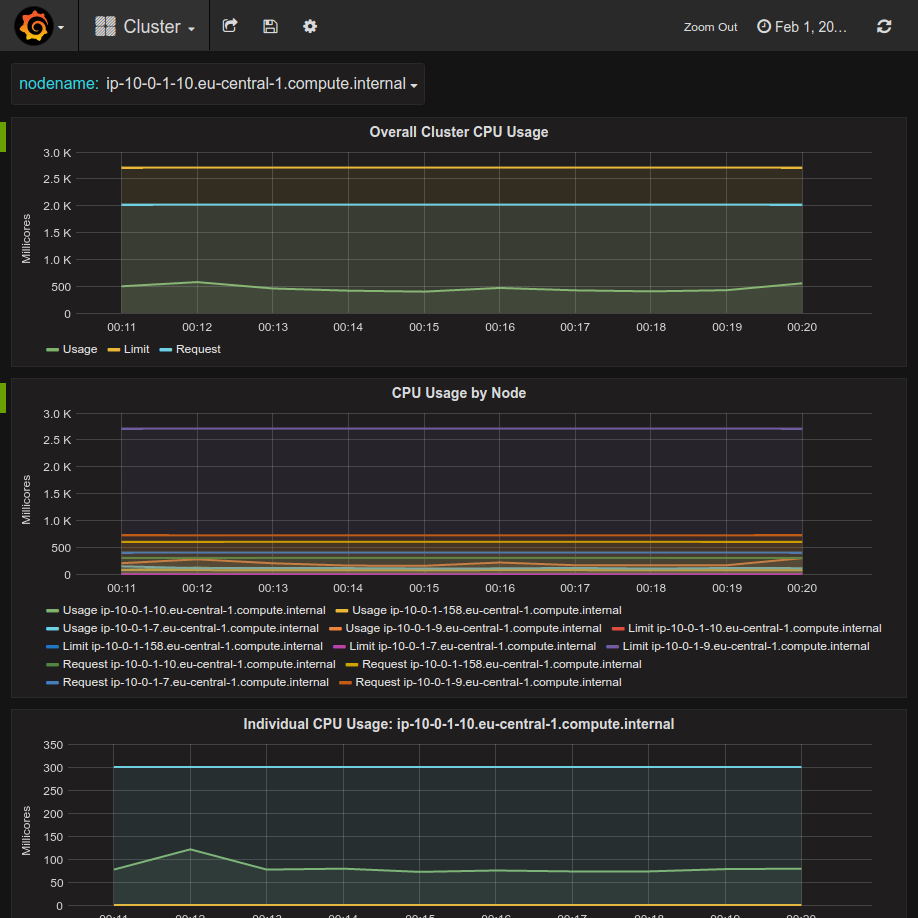
\includegraphics[width=1\textwidth]{grafana}
  \caption{Screenshot des Grafana Web-Interface}
  \end{figure}
\end{description}

\subsection{Alerting}

Sollten Metriken einen Anhaltspunkt f\"ur ein schwerwiegendes Problem geben,
m\"ussen die verantwortlichen Personen informiert werden.
Um diese Aufgabe zu erf\"ullen wird ein Alerting System integriert. In
diesem Fall wird Prometheus \cite{prometheus}
verwendet. Prometheus benötigt auf jeder einzelnen Node einen \quotes{Node exporter},
der die Metriken ausliest und an den Prometheus Prozess weiterleitet.
In Prometheus selbst können dann Bedingungen definiert werden, auf dessen Grundlage
Notifications versendet werden.

\begin{figure}[H]
\centering
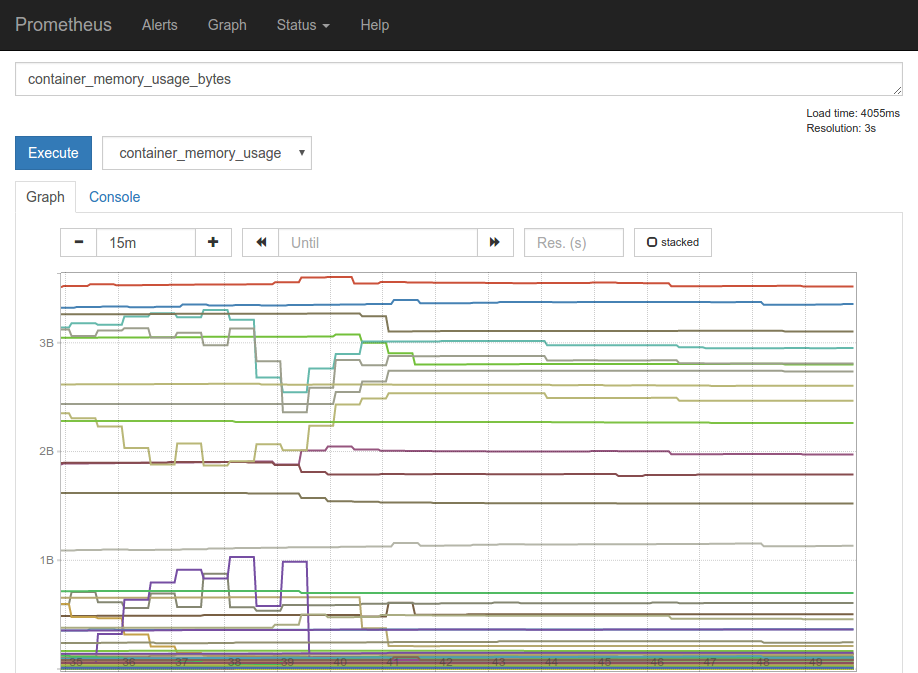
\includegraphics[width=1\textwidth]{prometheus}
\caption{Screenshot des Prometheus Web-Interface}
\end{figure}

\begin{tcolorbox}
Anmerkung: Mit dem ELK-Stack für das Logging, Grafana für das Monitoring und
Prometheus für das Alerting, sind drei wichtige Elemente für die Administration
des Clusters implementiert. Diese können dann nach außen hin freigegeben werden,
sodass auch Entwickler auf diese Informationen zugreifen können.
Wie diese Endpoints genau nach außen hin freigegeben und abgesichert werden,
wird in einem späteren Abschnitt erläutert.
\end{tcolorbox}

\section{Datenbank}

Da die Container in Kubernetes das Paradigma der Kurzlebigkeit und Ersetzbarkeit
erfüllen sollen, stellt sich die Frage, was mit Daten passiert, die nicht einfach
mit der Terminierung eines Pods verschwinden dürfen. Dies kann die Datenbank sein
oder auch ein Ordner, in dem beispielsweise User-Avatare als JPEG-Dateien abgelegt
werden.
Für die Applikation, die hier aber exemplarisch auf Kubernetes migriert werden soll,
handelt es sich um eine PostgreSQL Datenbank.

Der Anforderung, dass eine Datenbank aber persistent sein muss,
kann nun damit begegnet werden, dass sie nicht als
Teil des Clusters betrieben wird, sondern als separater Service.
Auf AWS würde dann hierfür die Verwendung des
\emph{Relational Database Service} (RDS)
in Frage kommen. Dies würde stärkeres Vendor Lock-in und höhere Kosten bedeuten
und wird deshalb an dieser Stelle vermieden.

Mit dem \emph{Persistent Volumes}-Feature in Kubernetes lassen sich
externe Datenträger einbinden.
Diese Volumes verschwinden nicht mit dem Verschwinden des Pods oder des
kompletten Clusters, sondern existieren weiter und können bei Bedarf mit
dem letzten Zustand wieder eingebunden werden.

Um nun also eine persistente Datenbank zu betreiben, wird der
Datenbank-Prozess als
Pod gestartet, der in sein lokales Filesystem das externe Volume
als Ordner einbindet. Um möglichst gute Latenzzeiten zu
erzielen, wird
für das \emph{Persistent Volume} ein \emph{Elastic Block Store} (EBS)
in derselben
Region und Availability Zone, in der auch das Cluster selbst liegt,
erstellt.

Die Instanzen, auf denen das \emph{Persistent Volume} eingebunden werden soll,
müssen mittels Terraform-Konfiguration die Rechte zum Einbinden dieses
Volumes per \emph{AWS-IAM Policy} zugewiesen bekommen
% cite https://adrianhesketh.com/2016/06/27/creating-aws-instance-roles-with-terraform/
.

\begin{lstlisting}[language=Python,numbers=none]
{
  "Effect": "Allow",
  "Action": "ec2:AttachVolume",
  "Resource": "*"
},
{
  "Effect": "Allow",
  "Action": "ec2:DetachVolume",
  "Resource": "*"
}
\end{lstlisting}

Nun kann Kubernetes mit folgendem \emph{Persistent Volume}-Spec auf
das EBS Volume
zugreifen:
\begin{lstlisting}[language=Python,numbers=none]
spec:
  capacity:
    storage: 10Gi
  accessModes:
    - ReadWriteOnce
  awsElasticBlockStore:
    volumeID: vol-03189b68f4c5cd7c8
    fsType: ext4
\end{lstlisting}

Der Pod muss dann dieses \emph{Persistent Volume} auf einem bestimmten Pfad
mounten, was in der folgenden Pod Konfiguration passiert.

\begin{lstlisting}[language=Python,numbers=none]
volumeMounts:
  - mountPath: /var/lib/postgresql/data
    name: pg-data\end{lstlisting}
\begin{lstlisting}[language=Python,numbers=none]
volumes:
  - name: pg-data
    persistentVolumeClaim:
      claimName: pg-data-claim\end{lstlisting}

Der Pod und die Node, auf dem die PostgreSQL-Datenbank für die zu
migrierende Applikation läuft, können nun ausfallen, ohne dass Daten verloren
gehen. Der Pod startet dann erneut und die alten Daten
in der Datenbank stehen sofort wieder allen Clients zur Verfügung.

Als zusätzliche Sicherheit vor fehlerhaften oder verlorenen Daten kann dann noch
ein weiterer Pod deployed werden, welcher in gewissen zeitlichen Abständen die
komplette Datenbank per \code{pg\_dump} in eine Datei extrahiert, welche dann
zum Beispiel verschlüsselt in einem S3-Bucket archiviert werden kann.

\section{API Deployment}

\subsection{Environment Variables}
Das bereits gebaute API-Image kann nun im Kubernetes-Cluster platziert werden.
Für diesen Zweck wird anstatt eines Replication-Controllers,
ein Deployment verwendet,
da so spätere Updates per \emph{Rolling Update} veröffentlicht werden können.
Die API braucht Zugang zur Postgres-Datenbank.
Gemäß dem \quotes{The 12-Factor App}-Grundsatz, werden die nötigen
Informationen für
den Datenbank-Zugriff (Credentials, Hostname, Port, Datenbank-Name)
per Environment-Variabel
gesetzt:
\begin{lstlisting}[language=Python,numbers=none]
env:
- name: POSTGRES_HOST
  value: criticalmaps-db
- name: POSTGRES_PORT
  value: "5432"
- name: POSTGRES_DB
  value: criticalmaps
- name: POSTGRES_USER
  value: foobar
- name: POSTGRES_PASSWORD
  value: 1337\end{lstlisting}

\subsection{Compute Resources}
Um die Funktionalität des \emph{Bin Packing} nutzen zu können,
muss Kubernetes wissen,
wieviel CPU und Memory der Container benötigt.
Hierfür stehen zwei verschiedene Direktive zur Verfügung.
Zum einen kann mit der \quotes{requests}-Direktive festgelegt werden
auf Grundlage
welcher Werte der \emph{kube-scheduler} die Container auf den Nodes
platzieren soll.
Sollte ein Container sich mehr Ressourcen nehmen, als in der
\quotes{requests}-Direktive
reserviert, passiert erst einmal noch nichts.
Mittels der \quotes{limits}-Direktive kann aber bestimmt werden,
ab wann ein Container
terminiert werden soll, sofern er zu viel CPU und/oder Memory konsumiert.
\begin{tcolorbox}
Hinweis: Zu hohe Last auf den einzelnen Containern soll über den
\emph{Horizontal Pod Autoscaler} ausgeglichen werden. Dieser wird in einem
späteren Abschnitt genauer behandelt.
\end{tcolorbox}
Die Terminierung der
Instanz mittels der \quotes{limits}-Direktive ist hier deshalb nötig, weil zu
hoher Ressourcen-Verbrauch auch andere Pods auf derselben Node in
Mitleidenschaft ziehen würde.

\begin{lstlisting}[language=Python,numbers=none]
resources:
  requests:
    cpu: 0.1
    memory: 200M
  limits:
    cpu: 0.2
    memory: 400M
\end{lstlisting}

Das Festlegen dieser Werte hängt zu einem großen Teil auch von Erfahrungen
vom Betrieb dieser Software unter realen Bedingungen ab.
An dieser Stelle soll eine
fundierte Entscheidung der initialen Werte für diese Konfiguration
begründet werden.

Um die oben getroffene Entscheidung zu erklären, soll hier nochmal erwähnt sein,
dass diese Container auf \code{t2.small}-Instanzen mit einer vCPU mit 3,3 GHz
und 2 GB Memory laufen. Mit \code{cpu: 0.1} fragt dieser Container 10\% der Leistung
dieser CPU an und \code{memory: 200M} meint 200 Megabyte des Arbeitsspeichers.

\emph{NodeJS} sollte pro Core mindestens einen Prozess (also Container) starten \cite{multicodenodejs}.
In diesem Fall also mindestens 1 Container.
Nach oben hin sollte die Anzahl nicht grundlos hoch sein, da dies den
\emph{Context Switching}-Overhead in der CPU erhöht \cite{nodejs}.
Weiter ist zu beachten, dass sich dieses Deployment die Node auch mit
anderen Containern
teilt und nicht alle vorhandenen Ressourcen verbrauchen darf.
Für eine gewisse Ausfallsicherheit, sollten also 3 Container per Host als Minimum
ausreichen. So wird dann erst einmal davon ausgegangen, dass 30\% der CPU und
circa 30\% RAM (also 600 Megabyte) ausreichen. Im Falle von plötzlich ansteigender
Last, kann dann 60\% der CPU und 60\% RAM (also 1.2 Gigabyte) genutzt werden,
bevor Kubernetes diese Pods terminiert und erneut startet.

In Verbindung mit dem \emph{Horizontal Pod Autoscaler} und
der \emph{AWS Auto Scaling Group}
kann so später sichergestellt werden, dass die Ressourcen auf den Nodes
effizient genutzt werden und bei Bedarf neue Nodes weitere
Ressourcen zur Verfügung stellen.

Es sollte allerdings keine CPU- oder Memory-Utilization von 100\% angestrebt werden,
denn so wäre kein Polster für weitere Nachfrage-Schwankungen gegeben.
Auch der Zeitraum, der benötigt wird, eine weitere Node zu starten, sollte
berücksichtigt werden, denn steigende Last kann nicht sofort, sondern erst
nach dem Boot und der Initialisierung der neuen Instanz
übernommen werden.

\subsection{Node Affinität}

Da die API-Container weder auf der Admin Node noch auf der Ingress Node
laufen sollen, muss auch dies per Pod-Manifest eingestellt werden.
Die Zeilen, die dafür sorgen, sind die Folgenden:

\begin{lstlisting}[language=Python,numbers=none]
nodeSelector:
  nodeRole: worker\end{lstlisting}

Der \emph{kube-scheduler} sorgt dann dafür, dass diese Pods nur auf den Nodes
landen, die diesem Label entsprechen.

In folgerndem Diagramm ist zu sehen, auf welchen Nodes die einzelnen Pods laufen.

\begin{figure}[H]
\centering
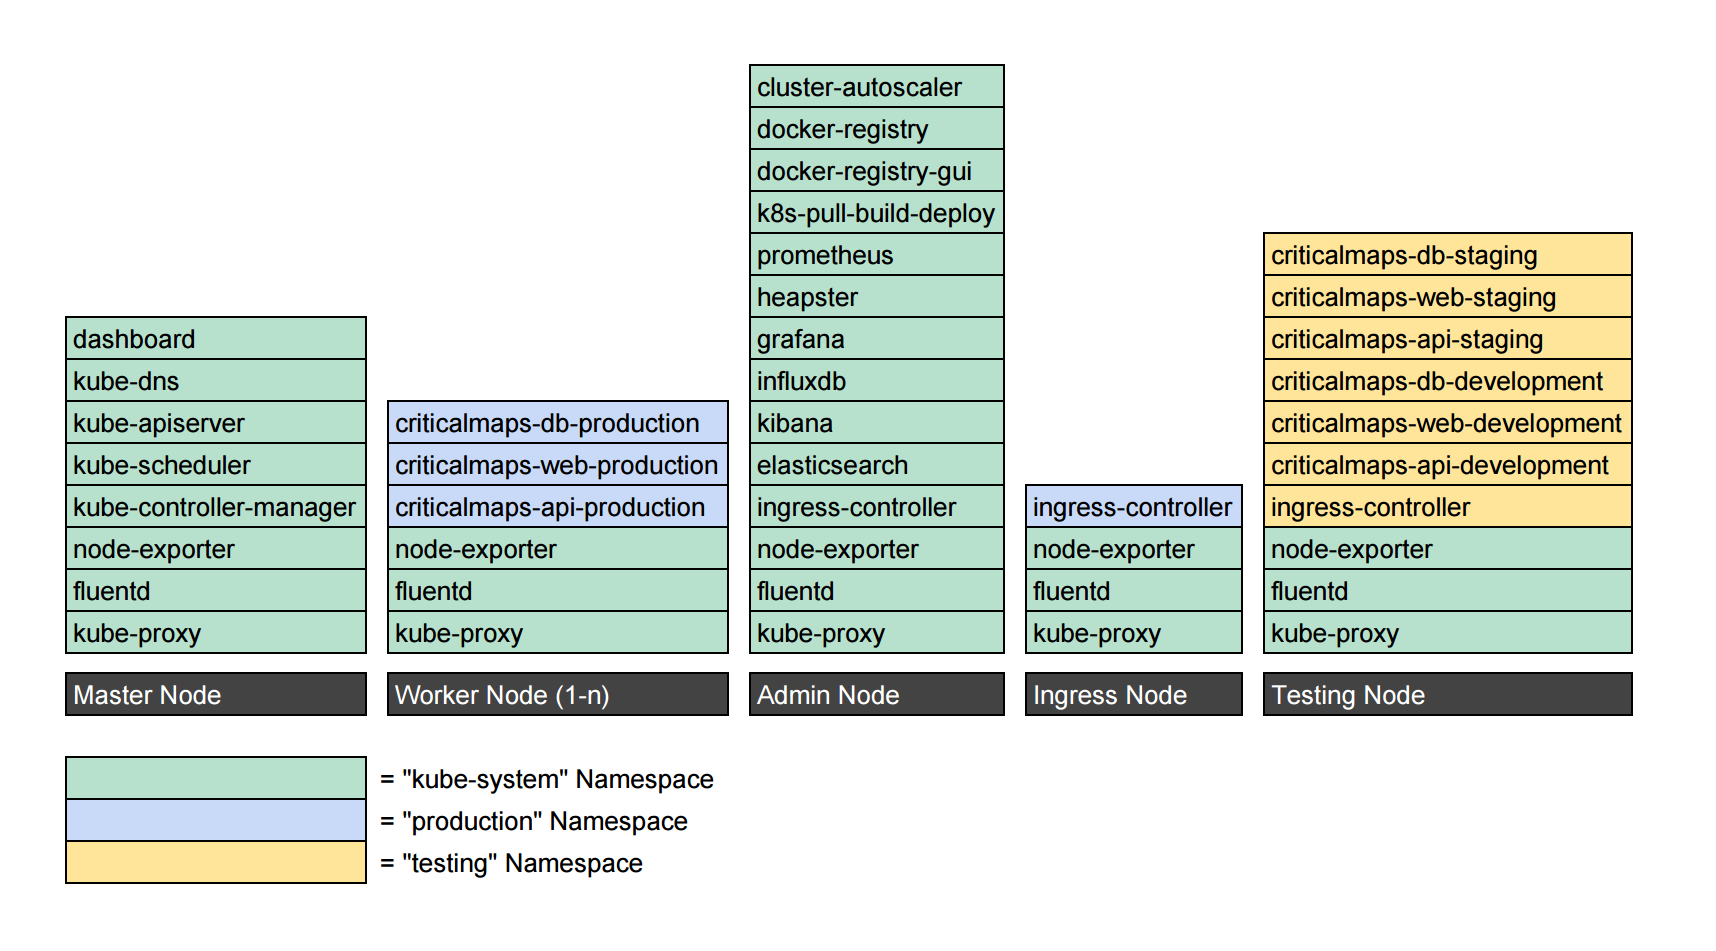
\includegraphics[width=1\textwidth]{namespaces}
\caption{Verteilung der Pods auf die einzelnen Nodes}
\end{figure}

\subsection{Horizontal Pod Autoscaler}

Der \emph{Horizontal Pod Autoscaler} ist ein Kubernetes Konfigurations-Element, mit dem
sich die Pods des gesamten Deployments überwachen lassen. Sollte die
durchschnittliche CPU-Utilization im Durchschnitt über alle Pods über
einen gewissen Wert steigen, werden zusätzliche Pods gestartet. Synchron dazu
werden Pods auch wieder gestoppt und gelöscht, wenn die CPU-Utilization unter
einen gewissen Wert fällt.

\begin{lstlisting}[language=Python,numbers=none]
minReplicas: 3
maxReplicas: 40
targetCPUUtilizationPercentage: 50\end{lstlisting}

Wenn also zu einem gewissen Zeitpunkt 50\% CPU-Utilization erreicht werden,
dann konsumieren alle Pods im Schnitt die Hälfte ihrer angefragten
CPU-Ressourcen.
Liegt dieser Wert der angefragten (also \code{requested}, nicht \code{limits}) CPU-Ressourcen
bei 10\%, dann bedeutet das,
dass der einzelne Pod von den jeweils 10\% angefragten CPU-Ressourcen
zu diesem Zeitpunkt 5\% benutzt.

Mit mindestens drei Pods startet diese Konfiguration. Sollten diese drei Pods
im Schnitt also über 50\% verbrauchen, wird ein weiterer Pod in das Deployment
hinzugefügt. Die Last wird nun also vom Service auf 4 Pods verteilt und die
durchschnittliche CPU-Utilization sollte wieder sinken.

Da aber eine Node nur beschränkte CPU-Ressourcen zur Verfügung stellt,
kann der \emph{kube-scheduler} weitere Pods nicht grenzenlos auf dieser Node unterbringen.
Wenn also jeder Pod 10\% anfragt, dann können nur 10 Pods per Single-Core Node
untergebracht werden. Um dieses Problem zu lösen, werden zwei
Techniken in einem späteren Abschnitt erörtert.

\section{Website Deployment}

Das Deployment der Website verhält sich synchron zu dem der API.
Aspekte wie die Konfiguration, Compute Resources, Node Affinität oder
der \emph{Horizontal Pod Autoscaler} können deshalb einfach von der API übernommen
werden und werden deshalb hier nicht erneut erörtert.

\section{Steuerung der Auto Scaling Group}

In einem voran gegangenen Abschnitt wurde eine \emph{Auto Scaling Group} erstellt.
Um nun über diese \emph{Auto Scaling Group} Instanzen zu starten und zu terminieren,
gibt es zwei Möglichkeiten, die im Rahmen dieser Arbeit umgesetzt
und evaluiert wurden.

Die eine Option wäre diese mittels AWS-Alarms vorzunehmen. Die andere ist, dass
in Kubernetes selbst ein Pod diese Vorgänge steuert.

\subsection{AWS-Alarms}

AWS-Alarms werden ausgelöst, sobald eine gewisse Metrik über oder unter einen
bestimmten Wert steigt oder sinkt. Wird der Alarm ausgelöst, kann eine
\emph{Scaling Policy} ausgelöst werden, welche dann die
\emph{Auto Scaling Group} anweist, nach oben
oder unten zu skalieren.
Zur Verfügung stehen die folgenden Metriken:

\begin{itemize}
  \item CPU Utilization
  \item Disk Reads
  \item Disk Read Operations
  \item Disk Writes
  \item Disk Write Operations
  \item Network In
  \item Network Out
\end{itemize}

Aufgrund der Charakteristika der zu deployenden Applikationen spielen
alle Disk-Metriken
eine eher unbedeutende Rolle.
Auch die Network-Metriken spielen keine große Rolle,
da sich hier unter normalen Bedingungen kein Performance-Flaschenhals
befindet.

Die bedeutsamsten Metriken, aufgrund derer eine Entscheidung über die
Skalieung getroffen werden kann, sind CPU- und Memory-Metriken.
Da AWS, aus Sicherheitsgründen, aber keine Memory-Metriken anbietet,
muss allein auf Grundlage der CPU-Metriken eine sinnvolle Scaling-Policy
gefunden werden.
\begin{tcolorbox}
  Hinweis: Theoretisch gibt es die Möglichkeit, diese Metriken über ein Script
  an \emph{AWS CloudWatch} zu senden und dann von dort zur Skalierung zu verwenden.
  Da aber ein Vendor Lock-in vermieden werden soll und diese Implementierung
  einen gewissen Aufwand und zusätzliche Komplexität darstellt,
  ist dieser Umweg hier keine Option.
\end{tcolorbox}
Das Feintuning dieser Policy hängt stark von der Art der Applikation
und dem Nutzungsverhalten ab.
Wird die Zahl der Instanzen zu schnell nach oben skaliert, werden eventuell
unnötigerweise zu viele Ressourcen vorgehalten.
Wird zu langsam hochskaliert, leidet die Response Time und damit
das \emph{User Experience}.

Durch mehrere Test haben sich folgende Regeln als sinnvoll erwiesen:
\begin{itemize}
  \item Füge eine weitere Instanz hinzu, wenn länger als 2 Minuten die
  CPU-Last über alle
  Instanzen höher als 50\% ist.
  \item Terminiere eine Instanz, wenn länger als 5 Minuten die
  CPU-Last über alle
  Instanzen geringer als 20\% ist.
  \item Nach jeder Skalierung, egal ob nach oben oder unten, darf 5 Minuten
  lang keine weitere Skalierung stattfinden.
\end{itemize}

Zudem darf die Anzahl der Instanzen, in diesem Fall, nicht höher als
8 sein. So wird verhindert,
dass sich die Anzahl der Instanzen Richtung Unendlichkeit hoch
skaliert,
nur weil ein Prozess außer Kontrolle geraten ist
und die CPU-Last in die Höhe treibt.

Im Folgenden ist nun die Konfiguration der Skalierung nach oben zu sehen.
Einfachheitshalber ist das Skalieren nach unten hier nicht zu sehen, denn es
verhält sich synchron zu diesem Beispiel.

Diese Alarm-Konfiguration:
\begin{lstlisting}[language=Python,numbers=none]
resource "aws_cloudwatch_metric_alarm" "high_cpu" {
  alarm_name          = "high_cpu"
  comparison_operator = "GreaterThanOrEqualToThreshold"
  threshold           = "50"
  statistic           = "Average"
  metric_name         = "CPUUtilization"
  namespace           = "AWS/EC2"
  evaluation_periods  = "2"
  period              = "60"
  alarm_actions       = ["${aws_autoscaling_policy.scale_up.arn  }"]

  dimensions {
    AutoScalingGroupName = "${aws_autoscaling_group.worker.name}"
  }
}\end{lstlisting}

löst dann diese Skalierunngs-Policy aus:
\begin{lstlisting}[language=Python,numbers=none]
resource "aws_autoscaling_policy" "scale_up" {
  name                   = "scale_up"
  scaling_adjustment     = 1
  adjustment_type        = "ChangeInCapacity"
  cooldown               = 300
  autoscaling_group_name = "${aws_autoscaling_group.worker.name}"
}\end{lstlisting}

Der Nachteil, der sich aus diesem Setup ergibt, ist, dass hier nur auf Grundlage
der abstrakten CPU-Utilization entschieden werden kann.
Diese AWS-Metriken kennen den internen Zustand des Clusters nicht.
Ein Herunterskalieren
würde auch bedeuten, dass eine Instanz, auf der zu diesem Zeitpunkt noch Pods
laufen, abrupt ausfällt und Kubernetes diese dann auf den übrigen Instanzen
starten muss. So kann es dazu kommen, dass beispielsweise laufende Requests
nicht beantwortet
werden. Zudem kann die Anzahl der Pods zwischen der Terminierung der
Instanz und dem
Starten der Pods auf einer der übrig geblieben Instanzen vorrübergehend
zu gering sein,
um die Last zu diesem Zeitpunkt abzudecken.

\subsection{Cluster Autoscaler Pod}

Der \emph{Cluster Autoscaler} ist ein Pod mit einem offiziellen Kubernetes Image aus dem
\quotes{contrib}-Repository \cite{contrib}. Dieser sitzt als weiterer Pod im
Cluster und überwacht die Ressourcen und die Nachfrage nach diesen.
Basierend auf diesen Daten, kann dann die \emph{Auto Scaling Group}
angesteuert werden.

\begin{description}
  \item[Wenn zu wenig Ressourcen zur Verfügung stehen:]
  Anders als der AWS-Alarm orientiert sich dieser Pod nicht an der tatsächlichen
  CPU-Utilization, sondern an der, die im Bin Packing für den Pod
  veranschlagt wurde.
  Um diese Logik verständlich zu machen, soll beispielsweise davon
  ausgegangen werden,
  dass nur eine Node existiert, auf der initial nur ein Pod mit 20\%
  CPU-Nachfrage läuft.
  Die Last steigt nun und der \emph{Horizontal Pod Autoscaler} muss weitere
  Pods starten,
  um die durchschnittliche CPU-Utilization über alle Pods dieses Typs auf
  einem gewissen Wert zu halten.
  Nach 5 Pods, die jeweils 20\% CPU-Ressourcen anfragen, kann
  der \emph{kube-scheduler}
  keine weiteren Pods mehr auf dieser Node platzieren, da die vorhandenen Pods
  bereits 100\% der CPU-Ressourcen reservieren.
  An dieser Stelle sendet der \emph{kube-scheduler} ein Event, auf das
  der \emph{Cluster Autoscaler Pod} registriert ist, um dieses Problem bekannt
  zu machen.
  Der \emph{Cluster Autoscaler Pod} steuert dann die \emph{Auto Scaling Group} an
  und startet eine weitere Instanz.
  Sobald diese gestartet ist, können auf dieser Node dann weitere
  Pods platziert werden. Der \emph{kube-scheduler} sorgt dafür, dass die Pods nun
  gleichmäßig auf den vorhandenen Nodes verteilt werden.
  Dieselbe Logik gilt hier natürlich synchron auch für Memory-Metriken.

  \item[Wenn zu viele Ressourcen zur Verfügung stehen:]
  Der \emph{Cluster Autoscaler Pod} überprüft in regelmäßigen Abständen auch, ob nicht
  zu viele Nodes im Cluster aktiv sind. Sollte dem so sein und sollten alle Pods
  einer speziellen Node auch Platz auf einer anderen Node finden, markiert
  der \emph{Cluster Autoscaler Pod}
  diese Node als Kandidat um terminiert zu werden.
  Als weiteren Schritt werden die Pods auf dieser Node auf andere Nodes verschoben.
  Der \emph{kube-scheduler} bringt diese auf einer der Nodes unter, die
  nicht terminiert werden sollen.
  Nach 10 Minuten wird die Node dann endgültig terminiert. Sollte sich aber
  während
  dieser 10 Minuten wieder eine Änderung der Last nach oben ergeben,
  die die vorhandenen Nodes nicht abdecken können, wird der komplette
  Terminierungsprozess abgebrochen und die Node wieder für Pods freigegeben.
\end{description}

Im Vergleich zum Ansatz per AWS-Alarm zu skalieren, berücksichtigt der Cluster
Autoscaler Pod auch Memory-Metriken.
Zudem lässt sich die Logik des \emph{Cluster Autoscaler Pod} gut mit der Logik des
\emph{Horizontal Pod Autoscaler} kombinieren und Terminierungen
von Nodes erfolgen
nicht so abrupt, sondern die Workloads der Node können im Vorfeld auf anderen
Nodes in Sicherheit gebracht werden.

Ein Nachteil dieses Ansatzes ist jedoch, dass die Instanz auf der Cluster
Autoscaler Pod spezielle IAM-Rechte zugewiesen bekommen muss.
\begin{lstlisting}[language=Python,numbers=none]
{
    "Effect": "Allow",
    "Action": [
        "autoscaling:DescribeAutoScalingGroups",
        "autoscaling:DescribeAutoScalingInstances",
        "autoscaling:SetDesiredCapacity",
        "autoscaling:TerminateInstanceInAutoScalingGroup"
    ],
    "Resource": "*"
}\end{lstlisting}

Dies könnte im Zweifel auch ein Angriffsvektor werden. Zudem sollte
erwähnt sein, dass der
\emph{Cluster Autoscaler Pod} noch keine ausreichenden
Möglichkeiten bietet,
um auch komplexere Szenarien abbilden zu können.
So sieht man in den Logs, dass der Pod scheinbar Schwierigkeiten mit der Existenz
der Admin-, Testing- und Ingress Node hat, welche keinen Einfluss auf die
Skalierungslogik haben sollten.
Wünschenswert wäre hier eine Einstellung, auf welche Nodes sich die
Skalierungslogik
bezieht, zum Beispiel per Label-Selektor.

Nichtsdestotrotz überwiegen die Vorteile des \emph{Cluster Autoscaler Pod}.
Die Logik, Skalierungen mittels AWS-Alarms vorzunehmen, kann aber als
Notfall-Ansatz beibehalten werden. Wenn dieser Alarm-Schwellenwert
auf sehr defensive
Werte eingestellt wird, sollte sicher gestellt sein, dass der
\emph{Cluster Autoscaler Pod} vorher reagiert. Sollte er das nicht tun, weil er
beispielsweise ausgefallen ist,
fängt der AWS-Alarm diesen Fall ab.

Es werden also beide Ansätze verwendet; Der \emph{Cluster Autoscaler Pod} und
für den Notfall
die AWS-Alarms, die bei über 80\% und unter 10\% CPU-Utilization reagieren.

\section{Ingress-Controller}

Um die unterschiedlichen Schnittstellen im Cluster nach außen hin, also für das
Internet freizugeben, bedarf es einer festen IP-Adresse, einem A-Record
Eintrag auf dem
DNS-Server, der auf diese IP-Adresse zeigt sowie einem Service, der die
TCP-Verbindungen auf Port 443 und
gegebenenfalls Port 80 annimmt und sie an den zuständigen Service weiterleitet.

Theoretisch, könnte man dafür auch einen Kubernetes \emph{Service}
benutzen, welcher folgende
Möglichkeiten bietet:

\begin{description}
  \item[Elastic Load Balancer:]
  Eine Option wäre den Service direkt mit einem externen
  Loadbalancer zu verbinden.
  Da sich das Cluster auf AWS befindet, wäre man hier an
   den \emph{Elastic Load Balancer} gebunden.
  Dieser würde zusätzliche Kosten verursachen und zu höherem
  Vendor Lock-in beitragen.
  \item[Node Port:]
  Der Service würde hier auf \textbf{jeder} Node denselben Port
  besetzen, welcher sich
  in der Port-Range von 30000 bis 32767 befindet, und damit nicht auf den
  Standard-Ports 80 und 443 laufen kann. Ohne zusätzliche Workarounds, könnte
  hier weder TLS-Terminierung, noch Authentifizierung stattfinden.
\end{description}

Diese beiden Optionen sind also eher unpraktikabel, weshalb eine weitere Option
evaluiert und umgesetzt wird.
Hierfür bietet es sich an, einen Ingress-Pod, der als Wrapper um \emph{Nginx}
deployed wird, zu benutzen.
Dieser Ingress-Pod belegt die Ports 80 und 443 auf
dem Netzwerk-Interface des Hosts,
nimmt Verbindungen entgegen, führt unter anderem
TLS-Terminierung und Basic-Auth durch und leitet diese Verbindungen dann weiter
auf den internen Service.
Sollte sich die interne Topologie ändern, ändert der Pod die
\emph{Nginx}-Konfiguration und lädt \emph{Nginx} mit dieser Konfiguration neu.

Da Verbindungen über HTTP auf Port 80 nicht verschl\"usselt sind, sollten
Requests auf diesen Endpoint idealerweise mit einem HTTP-Statuscode
\quotes{301 Moved Permanently}
beantwortet werden, der auf HTTPS auf Port 443 weiterleitet.

Alle Verbindungen landen so entweder direkt auf Port 443, der HTTPS anbietet, oder
werden auf diesen umgeleitet. In der Ingress-Konfiguration \cite{sslred}
passiert das \"uber folgende Annotation:

\begin{lstlisting}[language=Python,numbers=none]
ingress.kubernetes.io/ssl-redirect: "true"\end{lstlisting}

Bezüglich der Authentication unterscheiden sich hier zwei Fälle:
\begin{itemize}
  \item Der Endpoint benötigt keine Authentication oder die Authentication wird in
  der dahinter liegenden Applikation geregelt. Dies trifft zum Beispiel auf die API
  und die Website im \quotes{production} Namespace zu.
  \item Der Endpoint benötigt Authentication. Hierunter fallen zum Beispiel
  alle Frontend-Applikationen, die im Admin Namespace laufen.
\end{itemize}

Über die Ingress-Konfiguration lassen sich die Basic-Auth Credentials setzen,
indem ein Secret-Objekt erzeugt wird, welches Usernamen und Passwort als
\emph{base64}-encodierten \emph{.htaccess} String abspeichert.

\begin{lstlisting}[language=Python,numbers=none]
data:
  auth: c3RlcGhhbjokYXByMSRJZXdSUFcuZCR2azBiLjZvcWEuOUx5ZmtsM...\end{lstlisting}

Selbes gilt auch für das Zertifikat und den Key, die für die TLS-Termination
benötigt werden.

\begin{lstlisting}[language=Python,numbers=none]
data:
  tls.crt: LS0tLS1CRUdJTiBDRVJUSUZJQ0FURS0tLS0tCk1JSURFVENDQW...
  tls.key: LS0tLS1CRUdJTiBQUklWQVRFIEtFWS0tLS0tCk1JSUV2QUlCQU...\end{lstlisting}

Eine Schwierigkeit, in der Verwendung der Ingress-Controllers, ist, dass diese
jeweils nur mit Services verbunden werden können, die sich im selben Namespace
befinden.
Dieses Sicherheits-Feature verhindert dann, dass die
Staging- und die Development-Environment
über denselben Ingress-Controller angeboten werden können.
Für zwei Ingress-Controller für diese beiden Environments, bedarf es allerdings
auch zwei Nodes. Um Kosten für eine weitere Instanz zu vermeiden, sind in dieser
Umsetzung die Staging- und Development-Environment im selben Namespace
untergebracht,
welcher mit \quotes{Testing} benannt wurde.
Da diese beiden Environments nur Testzwecken dienen und damit wenig Last
verarbeiten müssen, ist dies eine sinnvolle Einsparungsmaßnahme.
Wünschenswert wäre zwar auch hier eine stärkere Isolation durch Namespaces,
jedoch ist dieser
Kompromiss hinzunehmen, da sich in diesen beiden Environments keine sensitiven
Daten, sondern nur Testdaten befinden sollen.

\begin{figure}[H]
\centering
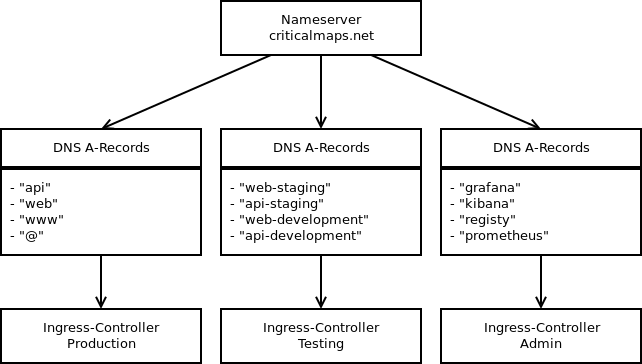
\includegraphics[width=0.8\textwidth]{dns}
\caption{Aufteilung der DNS A-Records auf die Ingress-Controller}
\end{figure}

\section{Docker Image Repository}

Um die Docker Images, die nicht direkt von externen Repositories
(wie Docker Hub oder Google Container Registry) heruntergeladen werden,
abzuspeichern und dem Cluster zur Verfügung zu stellen, gibt es zwei Möglichkeiten.

Die eine ist, einen externen Dienst zu benutzen, auf dem Images nicht-öffentlich
abgelegt werden. Die andere ist, so ein Repository im eigenen
Cluster zu betreiben. Da auch hier Kosten gespart werden sollen und die
Platzierung dieses Repositories direkt im Cluster für schnellere
Up- und Download-Zeiten sorgt, ist diese Option vorzuziehen.

\subsection{Docker Registry}

Für diesen Zweck stellt Docker ein Image bereit \cite{reg}.
Dieses Image wird auf der Admin Node in den \quotes{kube-system}-Namespace gestartet.
Der Container ist dann über Port 5000 erreichbar und sichert diese Verbindungen mit
TLS und Basic-Auth ab.

Da die Images, die in dieses Repository über die Zeit gepusht werden,
irgendwann für relativ hohen Speicherverbrauch sorgen können,
empfiehlt es sich, hierfür ein weiteres \emph{Persistent Volume} einzubinden. So
werden andere Pods auf der Admin Node nicht in Mitleidenschaft gezogen, sollte
die Festplatte irgendwann voll sein.

\subsection{Docker Registry GUI}

Der Umgang mit der API der Registry selbst ist relativ unhandlich und für
die Kontrolle der vorhandenen Images eher unpraktikabel.
Läuft die Registry auf dem Cluster, kann ein weiterer Pod genutzt werden, um
den Inhalt dieses Repositories in einer GUI im Browser anzuzeigen.

\begin{figure}[H]
\centering
\frame{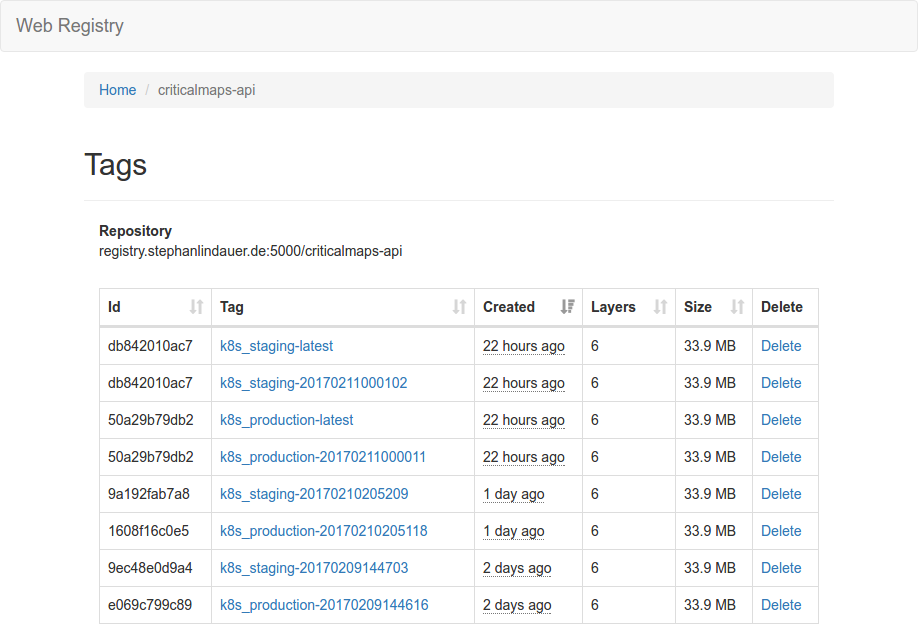
\includegraphics[width=1\textwidth]{registry-gui}}
\caption{Screenshot des Registry Web-Interface}
\end{figure}

Dieser wird wieder, wie andere Frontend-Komponenten, über einen
Ingress-Controller auf der Admin Node nach außen hin freigegeben.

\section{Continuous Deployment}

\subsection{Development Prozess}

Um die Pods, die die Domain-Logik abbilden, in die Continuous Delivery Pipeline
einbinden zu können, muss zuerst festgestellt werden, wie der Entwicklungsprozess
genau aussieht.
In dem Projekt, welches auf Kubernetes migriert wird, findet das \quotes{git-flow}-Pattern
Anwendung \cite{gitflow}.
Es gibt also unterschiedliche Git-Branches, die einen unterschiedlichen
Zweck erfüllen:
\begin{description}
  \item[Feature-Branches:]
  Hier werden neue Features entwickelt. Sobald diese fertig sind oder ein
  funktionierender Zwischenstand existiert, können diese auf den
  Development-Branch
  gemerged werden.
  \item[Develoment-Branch:]
  Hier werden die Feature-Branches immer wieder gemerged und damit zusammengeführt.
  \item[Release-Branches:]
  Auf diesen Branches werden Zwischenstände aus dem Development-Branch gemerged.
  Diese Zwischenstände sollen später automatisch gebaut und in die entsprechende
  Environment (\quotes{Development}, \quotes{Staging} oder
  \quotes{Production}) deployed werden.
  \item[Master-Branch:]
  Sobald der Production-Branch als erfolgreiches Deployment anerkannt wurde,
  wird dieser Zustand in den Master-Branch gemerged und mit einer
  Version getaggt.
\end{description}

Die folgende Grafik zeigt beispielhaft den Zusammenhang dieser einzelnen Branches
in dieser Umsetzung:

\begin{figure}[H]
\centering
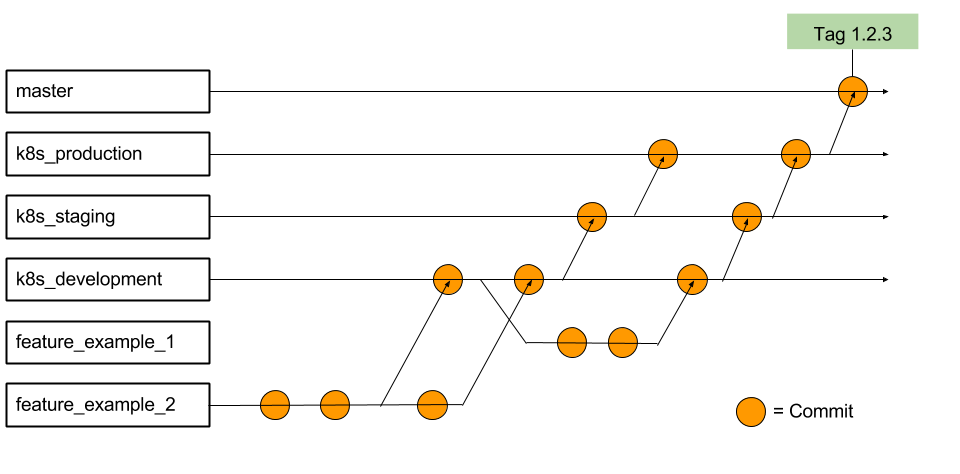
\includegraphics[width=1\textwidth]{k8s-gitflow}
\caption{Zusammenhang der Git-Branches}
\end{figure}

\subsection{Deployment Pipeline}

Um dieses Pattern anwenden zu können, muss Code aus den Release-Branches
automatisch im Cluster deployed werden, was folgende Schritte erfordert:

\begin{itemize}
  \item Der \code{HEAD} des Branches muss ausgecheckt werden
  \item Mit dem Dockerfile im root-Verzeichnis des Repositories wird ein Image gebaut
  \item Das Image wird getaggt und in das Docker-Repository gepusht
  \item Das Deployment für die jeweilige Environment macht ein \emph{Rolling Update}
  mit dem neuen Docker-Image
\end{itemize}

\subsection{Deployment Tools}

Um diese Schritte automatisch durchführen zu können, gibt es ein Vielzahl an
Möglichkeiten.

So könnte zum Beispiel ein Jenkins-Deployment diese Schritte cluster-intern
ausführen. Jenkins ist aber von seinem Funktionsumfang relativ ausgedehnt
\cite{continte}.
Die meisten der Jenkins-Features würden für diesen Use Case keine Anwendung
finden und trotzdem mehr Komplexität im Cluster-Management schaffen.

Eine weitere Alternative könnte ein externer Dienst wie Travis sein. Damit
Travis
aber diese Images bauen kann, braucht es Zugang zum Git-Repository. Um
dieses Image
dann im Cluster zu deployen, muss Travis darüber hinaus auch noch Zugang
zum Kubernetes
API-Server bekommen. Diese sicherheitstechnisch bedenklichen
Aspekte, die
erfahrungsgemäß langsamen Build-Jobs und der fehlende Cache für
die Docker-Layer
machen diese Option unattraktiv.

\subsection{Custom Deployment-Pipeline}

Da die Funktionalität dieser Deployment-Pipeline wenig komplex ist, ist im Rahmen
dieser Arbeit ein Script entstanden, welches genau diese Pipeline abbilden kann.

Wie viele andere Komponenten wird auch dieses Script als Pod deployed. Es muss
dafür also ein Docker-Image existieren, welches aber nicht in der eigenen
Registry liegen kann.
Der Grund hierfür ist, dass es sonst zu einem Henne-Ei-Problem kommen würde.
Wenn nämlich dieses Skript die zentrale Stelle sein soll, die Images baut, dann
kann sie sich nicht selbst bauen, da ohne den initialen Built dieses
Image gar nicht
existieren würde.
Um dieses Problem zu lösen, wird an dieser Stelle von der Vorgabe
abgewichen,
möglichst alle Aspekte innerhalb des Clusters selbst zu bereitzustellen.
Stattdessen kann an dieser Stelle das Docker Hub benutzt werden. Dieses erlaubt
registrierten Usern \textbf{eine} private, automatisierte Build-Pipeline
für Docker-Images, welche durch
Github-Commits ausgelöst wird.
So fallen durch Docker Hub keine weiteren Kosten an und sicherheitsrelevante
Konfigurationen können außerhalb dieses Images erst im Cluster selbst
eingebunden werden.
Für diesen Zweck sind auf Github und Docker Hub jeweils Projekte mit dem
Namen \quotes{k8s-pull-build-deploy} angelegt.

Die Wahl der Programmiersprache ist hier auf Ruby \cite{ruby} gefallen. Theoretisch kann
aber jede andere Sprache verwendet werden, die Shell-Befehle ausführen kann.

Das Dockerfile startet also vom \code{ruby:2.2} Base-Image.
Ruby kann so \quotes{out of the box} verwendet werden. Zusätzlich werden
folgende weitere Dependencies in das Image installiert:
\begin{description}
  \item[curl:] Um später die \code{kubectl}-Binaries
  herunterzuladen
  \item[git:] Um mit den Github-Repositories zu interagieren
  \item[kubectl:] Um direkt mit der Kubernetes-API über eine CLI kommunizieren
  zu können, anstatt die HTTP-Requests samt JSON-Objekte selbst zusammen zu bauen.
\end{description}

Eine weitere Dependency, die an dieser Stelle nicht installiert wird,
ist Docker selbst. Der Grund hierfür ist, dass es ein relativ großer Mehraufwand
wäre, Docker noch einmal in dem Image zu installieren, wenn es auf dem
Host-System bereits existiert.
Neben diesem Overhead gibt es weitere Gründe, keine
\quotes{Docker-in-Docker}-Lösung zu verwenden, welche Jérôme Petazzoni ausführlich
erörtert \cite{did}.
Damit der Container die Docker Komponenten des Hosts nutzen kann, werden diese
kurzerhand beim Starten des Containers in diesen hinein gemapped.
Konkret geht es um diese Pfade:
\begin{description}
  \item[/usr/local/bin/docker] Die Docker Binaries selbst, welche dann zum Beispiel
  \code{docker build} ausführen.
  \item[/var/run/docker.sock] Socket-Verbindung zum Docker Daemon auf
  dem Host-System.
  \item[/usr/lib/libdevmapper.so.1.02] Docker Dependency
\end{description}

Mit diesen Mappings kann der Container die Docker-Befehle auf dem Host
ausführen, ohne
dafür selbst Docker installieren zu müssen.

Weiter muss der Container in der Lage sein, mit dem Cluster per API-Server zu
kommunizieren.
Aus dieser Abhängigkeit ergibt sich die Frage, auf welcher Node der Container
am besten laufen soll.
\begin{description}
  \item[Master Node:] Auf der Master Node kann sich der Container ohne weiteres
  auf Port 8080 des \code{localhost}-Interface auf dem Host mit dem API-Server
  verbinden. Der Nachteil an dieser Lösung ist aber, dass das Bauen von Images
  keine Aufgabe der Master Node sein sollte, sondern eher auf die Admin Node passen
  würde. Da die Master Node eine so zentrale und wichtige Rolle im Cluster einnimmt,
  und dieser Container Ressourcen auf dieser Node verbrauchen würde,
  ist diese Lösung nicht zufriedenstellend.
  \item[Admin Node:] Im Sinne des \emph{Separation of Concerns}-Patterns,
  ist der Container hier bezüglich seiner Funktion besser aufgehoben.
  Um von hier aus mit dem API-Server auf Port 443
  zu kommunizieren, benötigt der Container auch Zugang zu den Zertifikat- und
  Key-Dateien, welche sich vom Host aus in den Container mappen lassen.
  Die Konfiguration wird hier also ein wenig komplexer.
  Der grösste Nachteil entsteht aber später in der initialen Bootstrap-Logik,
  worauf noch genauer eingegangen wird.
\end{description}

Die Konfigurations-Objekte für das Script sehen folgendermaßen aus:

\begin{lstlisting}[language=Python,numbers=none]
APPS = [
  {
    'name' => 'criticalmaps-api',
    'repository' => 'https://github.com/criticalmaps/criticalmaps-api.git',
    'build_branches' => [
      { 'name' => 'k8s_production',
        'namespace' => 'criticalmaps-production',
        'deployment_name' => 'criticalmaps-api',
        'deployment_image' => 'criticalmaps-api',
        'last_built_commit' => '' },
        # Weitere Branches hier ausgelassen
    ],
    'initial_clone_done' => false
  },
  # Weitere Applikationen hier ausgelassen
]
\end{lstlisting}

Wie zu sehen, wird das Repository sowie die einzelnen Branches
(hier: \quotes{k8s\_production}) und die dazu gehörigen Kubernetes Deployments
(hier: \quotes{criticalmaps-api} im Namespace \quotes{criticalmaps-production})
definiert.

Das Script führt ein \code{git clone} durch, sollte \code{initial\_clone\_done}
noch auf \code{false} stehen.
Es geht dann mit \code{git branch} durch die Branches und vergleicht
den \emph{SHA-1}-Hash
des \code{HEAD}-Commits mit der \code{last\_built\_commit} Variable, in der
abgespeichert wird,
welcher Commit dieses Branches bereits gebaut wurde.
Wenn der \emph{SHA-1}-Hash für diesen Commit noch nicht gebaut wurde,
wird dieser mit
\code{docker build} gebaut. Das Image wird
nach folgendem Schema getaggt:
\begin{lstlisting}[language=Python,numbers=none]
applikation:branch-latest
applikation:branch-timestamp
\end{lstlisting}
Am Beispiel der API würden diese Tags also in der Praxis so aussehen:
\begin{lstlisting}[language=Python,numbers=none]
criticalmaps-api:k8s_production-latest
criticalmaps-api:k8s_production-20170211000011
\end{lstlisting}
Das \quotes{latest} Image wird so immer wieder überschrieben, wobei aber die Images
mit dem Timestamp als Archiv im Repository verbleiben. So kann dann bei Problemen
mit der aktuellen Version des Images, manuell eine alte Version
deployed werden, ohne diese vorher bauen zu müssen.

Auf diese Weise kann ein \quotes{Poll for changes}-Mechanismus
\cite{duvall}
mit einfachen Mitteln umgesetzt werden.


\subsection{Bootstrapping der Manifeste}

Im Rahmen dieser Arbeit musste das Cluster immer wieder mit \code{terraform apply}
aufgesetzt und mit \code{terraform destroy} wieder zerstört werden. Wie bereits
erl\"autert, findet soweit bei der Erstellung des Clusters kein weiteres Bootstrapping der
Domain-Logik statt. So m\"ussten dann die ganzen einzelnen
\emph{YAML}-Manifeste vom Computer des Cluster-Admins, mit
\code{kubectl apply -f manifest-datei.yml} an die Kubernetes API übermittelt
werden. Dies bei jedem einzelnen Cluster-Neustart zu tun, ist repetitiv
und sollte automatisiert werden.
Das Aufsetzen eines komplett neuen Clusters wird ab dem Zeitpunkt, an dem
das Cluster in der Produktion eingesetzt wird, wahrscheinlich selten oder
gar nicht erfolgen. Für den Notfall, sollte aber selbst dann eine schnelle und
deterministische Möglichkeit bestehen, Manifest-Dateien an die Kubernetes-API
zu übermitteln.

Das Bootstrapping soll also am besten im Cluster selbst passieren. Zu
diesem Zweck wäre wieder ein Container wünschenswert, welcher im Cluster
sitzt und eine Verbindung zur Kubernetes-API aufbauen kann. Dasselbe Verfahren
wurde bereits bei der Umsetzung der \emph{Custom Deployment Pipeline} verwendet.
Auch hier muss das Image für diesen Container außerhalb des Clusters liegen,
da zu diesem Zeitpunkt ja noch kein Repository deployed wurde.

Für die Umsetzung dieses automatischen Bootstrappings kommen folgende
Verfahren in Frage:
\begin{description}
  \item[Auf der Master Node: ] Dies wäre die schnellste Variante, denn
  die Manifeste können sofort übertragen werden, sobald der API-Server
  bereitsteht. Die Umsetzung hierfür ist allerdings schwierig.
  Die Master Node ist eigentlich nicht dafür vorgesehen, Pods, außer den
  system-relevanten auszuführen, was durch die \code{SchedulingDisabled}-Flag
  deklariert wurde.
  Es gibt jedoch zwei Möglichkeiten trotzdem einen eigenen Pod auf der Master
  Node zu starten:
  \begin{description}
    \item[DaemonSet:] Ein \emph{DaemonSet} kann so definiert werden, dass es sich nur
    auf einer Node startet, indem über den \code{nodeSelector} eben nur diese
    eine Node ausgewählt wird. Das Starten dieses Pods würde dann über
    eine \emph{Systemd}-Unit geschehen, welche zuerst das \emph{Secret} für
    \emph{Docker Hub} per \code{curl} and die API weitergibt und dann das
    \emph{DaemonSet} selbst.
    Der große Nachteil hieran ist jedoch, dass ein \emph{DaemonSet} eigentlich ein
    Workload ist, der ohne zeitliche Einschränkung laufen soll. Der Zweck des
    Bootstrappings der Manifeste ist aber, diese an die API weiterzuleiten und
    danach zu terminieren. Ein \emph{DaemonSet} würde, wenn es terminiert, immer wieder
    neugestartet werden. Eine unschönes Workaround könnte es sein,
    den Container nach
    seiner Aufgabe einfach mit \code{sleep infinity} laufen zu lassen.
    \item[Pod:]
    Ein einzelner Pod kann auf der Master Node mittels eines Manifestes im
    \code{/etc/kubernetes/manifests}-Ordner automatisch gestartet werden. In
    diesem Ordner werden allerdings \textbf{nur} Pods gestartet. Alle weiteren
    Komponenten werden ignoriert.
    Da aber neben dem Pod auch noch ein \emph{Secret} deployed werden muss, damit
    das Image von Docker Hub geladen werden kann, bietet dieser Ansatz keine
    Lösung.
  \end{description}

  \item[Auf einer der Worker Nodes:]
  Wenn das Bootstrapping auf einer der Worker Nodes stattfindet, geht ein gewisser
  Zeit-Vorteil verloren. Denn so muss gewartet werden, bis auf
  der Worker Node, die Kubernetes-API erreichbar ist. Erst wenn dem so sein sollte,
  wird das \emph{kubelet} gestartet, welches dann die Anweisung vom
  \emph{kube-scheduler} bekommt, den Bootstrapping Pod zu starten.
  \begin{description}
    \item[Job:]
    Ein Job wäre für das Aktivieren der Manifeste eigentlich die richtige
    Komponente.
    In der Definition des Jobs kann festgelegt werden, dass der Container
    im Pod nur einmal laufen soll und nur neugestartet wird, wenn er
    nicht erfolgreich, also mit einem \emph{Exit code} ungleich 0, beendet.
    \item[Als Teil des \emph{Custom Deployment Pod}:]
    Der im vorangegangenen Abschnitt erstellte Pod, welcher das automatische
    Deployment regelt, hat die Abhängigkeit zu \code{kubectl} bereits
    installiert und konfiguriert.
    Das Bootstrapping kann also einfach vor dem Starten des automatischen
    Deployments stattfinden.
  \end{description}
\end{description}

Keine der oben genannten Optionen ist ohne Nachteile. Der Einfachheit halber
soll die Herangehensweise mittels des \emph{Custom Deployment Pod} weiter
verfolgt werden.
Der Ablauf des Bootstrappings ist also folgender:
\begin{itemize}
  \item Die Admin Node, auf der dieser Pod laufen soll, startet
  \item Die Admin Node stellt eine Verbindung zum API-Server her
  \item Kubelet startet
  \item \emph{kube-scheduler} startet Pod auf der Admin Node
  \item Pod startet mit \code{kubectl} alle Manifest-Dateien
\end{itemize}
